\documentclass[msc]{ppgccufmg}
\usepackage[english]{babel} % english | brazil
\usepackage[utf8x]{inputenc}
\usepackage[T1]{fontenc}
\usepackage{type1ec}
\usepackage{graphicx}
\usepackage[a4paper,
  portuguese,
  bookmarks=true,
  bookmarksnumbered=true,
  linktocpage,
  colorlinks, 
  citecolor=black,
  urlcolor=black,
  linkcolor=black,
  filecolor=black,
  ]{hyperref}
\usepackage[square]{natbib} %,numbers

% Additional Packages (Ueda)
\usepackage{tabularx}
\usepackage{scalerel}
\usepackage[dvipsnames]{xcolor}
\usepackage{nameref} % For cross-refering section titles
\usepackage{amsmath}
\usepackage{amssymb}
\usepackage{lmodern} % Cool font
\usepackage{multirow}

\include{definitions}

% Portuguese hyphenation causing problems in the English text
\hyphenation{re-qui-si-to}

\begin{document}

% O comando a seguir, \ppgccufmg, provê todas as informações relevantes para a
% classe ppgccufmg. Por favor, consulte a documentação para a descrição de
% cada chave.
\ppgccufmg{
  title={Reputation in Computer Science\\ 
      on a per Subarea Basis},
  authorrev={Ueda, Alberto Hideki},
  %cutter={D1234p},
  %cdu={519.6*82.10},
  university={Federal University of Minas Gerais},
  course={Computer Science},
  %portuguesetitle={Reputação em Ciência da Computação sob uma Perspectiva de Sub-Áreas},
  portugueseuniversity={Universidade Federal de Minas Gerais},
  portuguesecourse={Ciência da Computação},
  address={Belo Horizonte},
  date={2017-06},
  advisor={Berthier Ribeiro-Neto},
  coadvisor={Nivio Ziviani},
  abstract={Resumo}{resumo},
  abstract=[english]{Abstract}{abstract},
  dedication={dedication},
  ack={acknowledgements},   
  epigraphtext={And again when it shall be thy wish to end this play at night,\\
            I shall melt and vanish away in the dark,\\
            or it may be in a smile of the white morning,\\
            in a coolness of purity transparent.}
            {Rabindranath Tagore},%, Bengali poet}
%  epigraphtext={- Arrogance and fear still keep you from learning \\ 
%          the simplest and most significant lesson of all. \\
%        - Which is?\\
%        - It's not about you.}{Doctor Strange movie, 2016},
  indexkeys={1.~Computação --- Teses. 2.~Redes --- Teses. I.~Orientador.
    II.~Título.},
}

%%%%%%%%%%%%%%%%%%%%%%%%%%%%%%%%%%%%%%%%%%
\chapter{Introduction}
%%%%%%%%%%%%%%%%%%%%%%%%%%%%%%%%%%%%%%%%%%

Funding agencies, university officials, and department chairs constantly face the challenge of understanding how well the researchers they employ or sponsor are doing in terms of academic productivity and scientific impact. The assessment of their research quality usually includes the use of quantitative measures (e.g., citation counts, H-index) or qualitative surveys within their scientific community. For instance, in the United States (US), the National Research Council (NRC) applied in 2010 an extensive survey to gather information about more than one hundred US graduate programs. 

Overall, such assessments aim to capture the \textit{reputation} of each scholar or graduate program. That is, the perception of the researcher (or group of researchers) before the general public or before her (or its) academic peers. In principle, researchers with high reputation should receive priority treatment in the allocation of grants, research funds, scientific awards, and graduate students than less reputable ones within the same community.

However, even the aforementioned NRC attempt to present an evidence-based ranking of US graduate programs has not been accepted without controversy \citep{vardi17}. Additionally, allocating research funds with basis on an unidimensional ranking of graduate programs in a given area ignores the complex interplay between individual traits and program's unique patterns of strengths and weaknesses. While private organizations are also able to produce such rankings, it has been argued that in this way third-party business interests may influence academic values \citep{brembs13}.

In this dissertation, we provide a method for assessing the reputation of publication venues and graduate programs on a per subarea basis. For that, we rely on a reputation metric previously introduced in the literature \citep{ribas2015random} and modify it to the context of subareas. We apply this novel metric to rank conferences, journals, and graduate programs in Computer Science (CS) in Brazil and US.

%%%%%%%%%%%%%%%%%%%%%
\section{Motivation}
%%%%%%%%%%%%%%%%%%%%%

The decision of which researchers should be at the top --- for hiring, promoting, funding, or distributing grants, scholarships, awards and so on --- is typically based on criteria such as number of publications, impact of publications, number of undergraduate and graduate students under supervision, number of advised MSc and PhD theses, and participation in committees (conferences, program committees, journal editorial boards, technical committees, etc). 
%
Therefore, the effectiveness of the resulting ranking depends on how each criterion is assessed and the period of time covered in the assessment. Several indices have become widely used to measure the productivity of researchers. Examples include the raw number of citations, h-index ~\citep{hirsch2005}, g-index \citep{egghe2006theory} and citation z-score \citep{zscore}. Likewise, most academic search platforms, such as Google Scholar,\footnote{\url{http://scholar.google.com}} Microsoft Academic Search,\footnote{\url{http://academic.research.microsoft.com}} and AMiner\footnote{\url{http://arnetminer.org}} use some of such indices to rank researchers.

However, ranking researchers without regarding the specificity of their subareas or sub-fields of research is arguably unfair and potentially error-prone \citep{lima2013jcdl}. For instance, consider the problem of comparing the research output of two different researchers, where the first one works on a subarea $A$ and the second one works on a subarea $B$. If we assume that it is inherently harder to publish articles in $A$ than in $B$, it seems natural that the metrics used to rank these researchers should be distinct, or, at least, take those differences between subareas into account. Otherwise, the comparison between them would be unfair.

As an illustration, consider the subarea of Human-Computer Interaction within the broad field of CS. Experimental evaluation in this area usually takes more time than in other CS subareas when arranging and assessing users' feedback is necessary~\citep{wainer13}.
%
On the other hand, CS subareas such as Databases and Computer Graphics do not usually face the same problem because their experimental evaluations depend on assessing the outcome of an automatic process, such as a query evaluation or a graphics rendering engine. Likewise, researchers from some subareas may have fewer publications than others, but with a potentially higher impact in their community. 

To have a better understanding of this current problem in academic rankings, see the scenario of CS in Table \ref{tab:subareas-list}.  It contains a list of 37 subareas of Computer Science according to Microsoft Academic Search. Although many studies in the literature show that there are significant differences in CS subareas' publication patterns \citep{hoonlor13,lima15,wainer13}, several institutions responsible for evaluating graduate programs do not take those differences into account. 

\begin{table}[htbp]
  \centering
  \caption{The Microsoft 37 Subareas of Computer Science}
  \label{tab:subareas-list}
  \begin{tabular}{ll}
    \toprule
    \multicolumn{2}{c}{CS Subareas}\\
    \midrule
    Algorithms & Internet privacy \\
    Artificial intelligence & Knowledge management \\
    Bioinformatics & Machine learning \\ 
    Cognitive science & Management science \\ 
    Computational biology & Mathematical optimization \\ 
    Computational science & Multimedia \\ 
    Computer architecture & Natural language processing \\ 
    Computer graphics & Operating systems \\ 
    Computer hardware & Operations research \\ 
    Computer networks & Parallel computing \\ 
    Computer security & Pattern recognition \\ 
    Computer vision & Programming languages \\ 
    Data mining &  Real-time computing \\ 
    Data science & Simulation \\ 
    Databases & Speech recognition \\ 
    Distributed computing & Telecommunications \\ 
    Embedded systems & Theoretical computer science \\ 
    Human-computer interaction & World Wide Web \\
    Information retrieval \\
  \bottomrule
\end{tabular}
\end{table}

{\color{blue}
In Brazil, for instance, as in several other countries, the graduate programs are evaluated by a funding agency. This agency, called CAPES,\footnote{Foundation for the Coordination and Improvement of Higher Level or Education Personnel. \url{http://capes.gov.br}} runs periodic evaluations of graduate programs and uses citation-based metrics to rank all publication conferences and journals. Specifically, it ranks the graduate programs based on their publication records and other features such as courses taught, number of students graduated, average time to graduate a student, and department infrastructure. In this evaluation model, the ranking of publication venues is decisive on identifying the most reputable graduate programs. Thus, if the ranking of venues does not take into account the differences in subareas, the evaluation of graduate programs runs the risk of being very biased towards criteria such as popularity or raw publication volume~\citep{capes09}.

Moreover, the distribution of grants, scholarships, and awards, among others benefits for individual researchers, are also computed from the perspective of the broad areas. Further, funding agencies as CNPq\footnote{Brazilian National Research Council. \url{http:/cnpq.br}} impose quantitative limits on the members of the highest grants (or productivity levels) issued to any given broad area of knowledge, such as CS~\citep{capes17}. It so, one can realize that the most popular subareas in CS have large advantages in this classification process over the other subareas in CS. 
%
%For instance, the subarea of Computational Theory cannot be equally compared to Data Mining, since the latter has more researchers, publications, and venues available today than the former one. 
%
Therefore, there is a necessity of a closer look to these academic scenarios from a perspective of subareas.
}

%%%%%%%%%%%%%%%%%%%%%
\section{Dissertation Statement}
%%%%%%%%%%%%%%%%%%%%%

We claim that general purpose rankings of CS graduate programs, % in Brazil, 
rankings based on weights associated with the venues in the broad area of knowledge without consideration to particularities of subareas, may not reflect important information about the academic excellence of these programs. For instance, if the government intends to stimulate research groups working on a specific subarea, such as Machine Learning, a general ranking in the broad area of CS will not facilitate the decision. 

In particular, this dissertation aims to answer the following research questions:
    
\begin{itemize}
    \item Q1. How to quantify the reputation of publication venues and graduate programs on a per subarea basis?     
    \item Q2. How does the reputation of Brazilian and US graduate programs in CS vary per subarea?     
    \item Q3. Are there differences between the current research directions in CS of the top Brazilian and US graduate programs?
\end{itemize}

%% How we answered those questions?
To answer these questions we extend the usability of a reputation metric called P-Score (for Publication Score)~\citep{ribas2015bigscholar} proposed in the literature. We apply this extended metric in an academic dataset to produce rankings of publication venues and graduate programs in CS on a per subarea basis. Then, we analyze the reputation of Brazilian graduate programs in CS by subarea and compare them to US graduate programs working in the same subareas. We also provide an overview of current research directions of the two countries, i.e., on which subareas they have the most prominent work nowadays.

\newpage

%%%%%%%%%%%%%%%%%%%%%
\section{Contributions}
%%%%%%%%%%%%%%%%%%%%%
Our main contributions are:

\begin{itemize}
    \item Contribution 1: A novel reputation metric for academic rankings on a per subarea basis.
    \item Contribution 2: An analysis of research output in Computer Science in Brazil and US on a subarea level.
    \item Contribution 3: A comparison between the current research directions in CS of Brazil and US and insights on the differences in research interests of each country.
\end{itemize}

%%%%%%%%%%%%%%%%%%%%%
\section{Dissertation Overview}
%%%%%%%%%%%%%%%%%%%%%
The remainder of this dissertation is structured as follows. In Chapter \ref{sec:related} (\nameref{sec:related}), we present a literature review on reputation models and some instantiations of these models in academic search tasks. Chapter \ref{sec:pscore} (\nameref{sec:pscore}) describes the theoretical concepts supporting our approach, by presenting the key ideas of the reputation model we used in this work and the strategies we adopted to study the academic data on a per subarea basis. In Chapter \ref{sec:setup} (\nameref{sec:setup}), we present the experimental methodology of our reputation assessment, including information about our academic dataset, ground-truths considered and evaluation metrics we adopted in this study. Chapter \ref{sec:results} (\nameref{sec:results}) discusses our findings on ranking publication venues and CS graduate programs from Brazil and US, and presents a comparison between the scientific directions of the two countries. Chapter \ref{sec:conclusions} (\nameref{sec:conclusions}) concludes the dissertation, summarizes the key contributions of this work and provides directions for further research.


%%%%%%%%%%%%%%%%%%%%%%%%%%%%%%%%%%%%%%%%%%
\chapter{Related Work}\label{sec:related}
%%%%%%%%%%%%%%%%%%%%%%%%%%%%%%%%%%%%%%%%%%

In this chapter, we describe related work on academic search considering the broad areas of knowledge (Section~\ref{sec:rwbroad}) and on a per subarea basis (Section~\ref{sec:rwsubarea}).

% Citation-based metrics have been widely applied to rank computer and information science journals~\citep{Katerattanakul2003,nerur2005assessing}. Also, different approaches using citation data have been proposed to measure the quality of publication venues in the Databases subarea~\citep{rahm2005citation} and to rank documents retrieved from a digital library~\citep{larsen2006using}. 

%%%%%%%%%%%%%%%%%%%%%
\section{Academic Search in Broad Areas}\label{sec:rwbroad}
%%%%%%%%%%%%%%%%%%%%%

Garfield's Impact Factor~[\citeyear{garfield1955}] is one of the first metrics proposed to quantify research impact. It has been widely used nowadays to measure relative importance of a scientific journal within its field. In a nutshell, it indicates the average number of citations per publication of a journal, in the last two years.  Despite its wide usage since it was proposed in 1955, it has been largely criticized~\citep{saha2003}. 
%
Accordingly, several alternatives have been proposed in the literature, such as other citation-based metrics \citep{egghe2006theory,waltman11,sun2007popularity,waltman11,yan2011p,zscore}, download-based metrics~\citep{bollen2005toward}, PageRank-like metrics~\citep{gollapalli2011ranking,Yan:2007}, and community-based features \citep{Silva14}. 

One of the most widespread citation-based metric, the H-index, was proposed by \cite{hirsch2005}. It has been mainly used to rank researchers both in terms of productivity and scientific impact. The key idea behind the H-Index is to detect the number of publications of high impact an author has in her research career --- for instance, penalizing authors with a large volume of articles but with a low number of citations for the majority of them. Additionally, several works proposed different uses of citation data ~\citep{ding2011,egghe2006theory,sun2007popularity,yan2011p} and studied their impact, advantages, and disadvantages~\citep{martins2009,leydesdorff2009new}.

The idea of reputation, without the direct use of citation data, was discussed by \cite{nelakuditi2011snap}. They proposed a metric called \textit{peers' reputation} for research conferences and journals, which ties the selectivity of the publication venue based upon the reputation of its authors' institutions. The proposed metric was shown to be a better indicator of selectivity of a research venue than acceptance ratio. In addition, the authors observed that, in the subarea of Computer Networks, many conferences have similar or better peers' reputation than journals. This result is similar to the conclusions obtained by \cite{laender2008}, who show that conference publications are important vehicles for disseminating CS research, while in other areas such as Physical Science and Biology the most relevant venues are arguably the scientific journals.

%% Expert Search
Regarding the assessment of individual researchers' influence and expertise, many approaches have been introduced~\citep{balog2012ftir, cormode2014people, deng2012modeling, gollapalli2011ranking, wu2009detecting}. Particularly, \cite{goncalves2014} quantified the impact of various features on a scholar popularity throughout her career. Specifically, they analyzed how features that capture the number and rate of publications, number and quality of publication venues, and the importance of the scholar in the co-authorship network relate to the scholar popularity, by applying regression analysis. They concluded that, even though most of the considered features are strongly correlated with popularity, only two features are needed to explain almost all the variation in popularity across different researchers: the number of publications and the average quality of the scholar’s publication venues. This finding is one of the hypotheses for the reputation model introduced by Ribas et al.~[\citeyear{ribas2015random}]. 

%% Prediction
In addition, the prediction of scientific success of a researcher is also valuable for several goals, for example, hiring faculty members, guiding funding agencies in their decision processes and improving scholar rankings in academic search engines \citep{masoumeh16}. As a result, previous work attempted to predict if a researcher will become a principal investigator~\citep{vandijk14}, her future H-index~\citep{dong15, penner13} and the potential number of citations to her publications~\citep{castillo2007estimating,mazloumian12}.

Although citation-based metrics are useful, they are not enough to do a complete evaluation of research.  In particular, \cite{piwowar2013altmetrics} showed that metrics as the H-Index are slow, as the first citation of a scientific article can take years. He concludes that the development of alternative metrics to complement citation analysis is not only desirable, but a necessity.

The reputation model we use in this work was proposed by Ribas et al.~[\citeyear{ribas2015random}]. This model, called \textit{reputation flows}, exploits the transference of reputation among entities in order to identify the most reputable ones. Particularly, the reputation flows consist in a random walk model where the reputation of a target set of entities is inferred using suitable sources of reputation. To evaluate this model, they instantiated the reputation flows in an academic setting, proposing a novel metric for academic reputation, the \textit{P-score}~\citep{ribas2015bigscholar}. Instead of relying on standard citation-based approaches for identifying reputable venues and researchers, P-score captures publishing behavior as a reputation signal, using a few highly reputable sources (e.g., reputable publication venues). For a better understanding of both the extension we propose and the methodology we adopted in this work, we provide in Chapter~\ref{sec:pscore} more detailed information about the \textit{reputation flows} model and its instantiation in the academic domain. 

%% Studies on a per Subarea Basis
By and large, the aforementioned works or variations of them are commonly used in assessments of academic output and also by modern search engines for scientific digital libraries, such as Google Scholar\footnote{\url{https://scholar.google.com.br}}, Microsoft Academic Search\footnote{\url{http://academic.microsoft.com}}, AMiner\footnote{\url{http://aminer.org}}, %maintained by \cite{Tang:08KDD},
and CiteSeerX\footnote{\url{http://citeseerx.ist.psu.edu}}.  
%, directed by \cite{citeseerx},
% Semantic Scholar~\footnote{\url{http://semanticscholar.org}}, mantained by the Allen Institute for Artificial Intelligence,
% CS Rankings~\footnote{\url{http://csrankings.org}}, maintained by Berger of the University of Massachussets.
However, none of the referred metrics take into account the different publication patterns in the subareas. Studies suggesting those differences and the negative impact of uniform evaluation metrics have been discussed in the field of Economics~\citep{kapeller10, lee10} and in Computer Science~\citep{hoonlor13, laendersigs15, lima2013jcdl}.

%%%%%%%%%%%%%%%%%%%%%
\section{Academic Search on a per Subarea Basis}\label{sec:rwsubarea}
%%%%%%%%%%%%%%%%%%%%%

% Laender sigs-graph Clustering
\cite{alves} and \cite{laendersigs15} analyze the structure of the communities formed by the flagship conferences of ACM SIGs. Their findings show that most of the ACM SIGs are able to connect their main authors in large and visually well-structured communities. However, they note that a few conferences, such as the ACM Symposium on Applied Computing, flagship conference of SIGAPP, and the ACM Conference on Design of Communications, flagship conference of SIGDOC, do not form a strong research community, presenting a structure with several disconnected components. They have opened their results to the research community as an interactive visualization tool\footnote{\url{http://acmsig-communities.dcc.ufmg.br}} that allows one to browse the scientific communities, visualizing their structures and the contribution of each specific researcher to connect its coauthorship graph. The concept of scientific community and its natural development enforced the clustering approach we initially adopted in this work.

Several comparative studies on research productivity between nations have been presented, for improving evaluation metrics \citep{laender2008}, characterizing research development in different regions of the world \citep{menezes09}, or suggesting directions to improve scientific production and impact \citep{wainer09}. In constrast with these aforementioned works, we are the first to perform this comparison using the reputation model proposed by Ribas et al.~[\citeyear{ribas2015random}] and its derived metric, called P-score. %We provide more details of this model in Chapter \ref{sec:pscore}.

\cite{lima2013jcdl} showed how important the subareas of expertise are when assessing research profiles in Computer Science, proposing the \textit{ca-index}, a cross-area metric for ranking researchers by aggregating their productivity indexes across multiple areas. Likewise, they aimed to improve the reputation assessment of authors with interdisciplinary research output. In contrast, we propose to assess reputation of researchers in each CS subarea independently, treating each subarea as a different research community.

\cite{wainer13} presented the first attempt to quantify the differences in publication and citation practices between the subareas of Computer Science. Their key findings were: i) there are significant differences in productivity across some CS subareas, both in journals (e.g., Bioinformatics has a significantly higher productivity than Artificial Intelligence) and in conferences (e.g., Image Processing and Computer Vision has a significantly higher productivity than Operational Research and Optimization), ii) the mean number of citations per paper varies depending on subarea (e.g., Management Information Systems has significantly higher citation rates per paper than Computer Architecture), and iii) there are significant differences in emphasis on publishing in journals or in conferences (e.g., Bioinformatics are clearly journal oriented while Artificial Intelligence are conference oriented). However, they do not focus on modeling a new productivity metric for academic domain taking into account those differences between the subareas.

{\color{blue} 
The idea of using normalized metrics to assess reputation of academic entities, on a per subarea basis, was inspired by previous works in the literature~\citep{leydesdorff13,glanzel11,opthof10,waltman13}. Such metrics were proposed to consider the differences in publication and citation practices among research subareas.

To the best of our knowledge, this is the first work that tackles the problem of both identifying the most important venues of a subarea in Computer Science and ranking graduate programs based on this information, in a semi-automatic fashion.
}

% ,raan10,smolinsky16
% http://aclweb.org/anthology/D/D16/D16-1142.pdf
% The Ranking Competition Between Publishers, Nimrod Raifer, Fiana Raiber, Moshe Tennenholtz and Oren Kurland

%%%%%%%%%%%%%%%%%%%%%%%%%%%%%%%%%%%%%%%%%%
\chapter{Reputation Flows and P-score}\label{sec:pscore} 
%%%%%%%%%%%%%%%%%%%%%%%%%%%%%%%%%%%%%%%%%%

In this chapter, we describe the reputation model we adopted as reference and the modifications we propose to it, in order to obtain rankings of academic entities on a per subarea basis. Specifically, in Sections \ref{sec:flows} and \ref{sec:spscore}, we summarize the key points of the Reputation Flows' model and its derived metric for academic search, the P-score, proposed by \cite{ribas2015bigscholar}. This introduction is essential to comprehend the modifications we propose for the reputation model to take subareas into account. The motivation for such adjustments is described in Section \ref{sec:encroachment}. Then, in Sections \ref{sec:npscore} and \ref{sec:wpscore}, we discuss in detail our ideas to consider a per subarea basis and the specific modifications aimed towards this purpose.

%%%%%%%%%%%%%%%%%%%%%
\section{Reputation Flows}\label{sec:flows}
%%%%%%%%%%%%%%%%%%%%%

While quantifying the reputation of a given entity is a challenging task, \cite{ribas2015random} argue that the flow of reputation among entities can be accurately modeled as a stochastic process. To this end, they proposed a conceptual framework for ranking entities that convey reputation to one another. They introduced a \textit{reputation graph}, a data structure that models the flow of reputation from selected sources to multiple targets and then formalized a stochastic process to estimate the amount of reputation transferred to target entities. This model was called \textit{reputation flows}.

\begin{figure}[h]
   \centerline{
\includegraphics[width=.7\linewidth]{fig/overview-line}}
   \caption{Structure of the reputation graph.}
   \label{fig:rgraph}
\end{figure}

The interaction between reputation sources and reputation targets is inspired by the notion of {\em eigenvalue centrality} in complex networks, which also provides the foundation to PageRank~\citep{brin98}. In particular, let $S$ be the set of reputation sources, $T$ the set of reputation targets, and $\bP$ be a \emph{stochastic} matrix of size $(|S|+|T|) \times (|S|+|T|)$ with the following structure: 

\newcommand{\bkt}[1]{ {^{\langle #1 \rangle}} }

\begin{align}\label{eq:newp}
%\[
\bP =
\left[
\begin{array}{r | r}    
    \delta_{s} \cdot \underset{S \times S}{\bP_1} \ \ & (1-\delta_{s}) \cdot \underset{S \times T}{\bP_2} \\ 
    \hline
    (1-\delta_{t}) \cdot \underset{T \times S}{\bP_3} \ \ & \delta_{t} \cdot \underset{T \times T}{\bP_4} \\
\end{array}
\right],
%\]
\end{align}
\noindent where each quadrant represents a distinct type of reputation flow. Matrix $\bP$ depends on the following matrices:

\begin{itemize}
    \item $\bP_1$: stochastic matrix of size $|S|\times |S|$ representing the transition probabilities between reputation sources;
    \item $\bP_2$: matrix of size $|S|\times |T|$ representing the transition probabilities from reputation sources to targets;
    \item $\bP_3$: matrix of size $|T|\times |S|$ representing the transition probabilities from reputation targets to sources;
    \item $\bP_4$: stochastic matrix of size $|T|\times |T|$ representing the transition probabilities between reputation targets.
\end{itemize}

The parameters $\delta_{s}$ and $\delta_{t}$ control the relative importance of the reputation sources and targets, which are modeled in the four matrices above. Specifically, $\delta_{s} \in [0,1]$ is the fraction of reputation one wants to transfer between source nodes and $\delta_{t} \in [0,1]$ is the fraction of reputation one wants to transfer between target nodes. These parameters are useful to calibrate the impact of different types of reputation flows in the final reputation score.

Note that, as ($i$) the sub-matrices $\bP_1$ and $\bP_4$ are \emph{stochastic} and ($ii$) each of the rows of matrices $\bP_2$ and $\bP_3$ sums to 1, then $\bP$ defines a Markov chain. Assuming that the transition matrix $\bP$ is ergodic, we can compute the steady state probability of each node and use it as a reputation score.%
%
\footnote{Recall that, in an ergodic process, the state of the process after a long time is nearly independent of its initial state.~\citep{walters00}}
%
Specifically, we can obtain values for ranking the set of nodes by solving:

\begin{align}
\label{eq:ggP}
    \bpi = \bpi \bP,
\end{align}
\noindent where $\bpi$ is a row matrix with $|S|+|T|$ elements, each one of them representing the probability of a node in the set $S \cup T$. This system of linear equations can be solved by standard Markov chain techniques, as the Power Method.\footnote{\url{http://en.wikipedia.org/wiki/Power_iteration}} Then, we obtain the steady state probabilities of all nodes in $S \cup T$ (reputation sources and reputation targets).

In short, the steady state probability of an entity is interpreted as its relative reputation, as transferred from other entities in a reputation graph. Subsequently, the reputation of the target nodes can be further propagated to entities we want to compare, in the \textit{collateral set} $C$, as shown in Figure~\ref{fig:rgraph}. 
%
% The use of collaterals allows us to isolate the impact of a set of arbitrary nodes on the reputation graph, fixing reputation sources as the only set of nodes providing reputation. While this design choice aimed primarily at effectiveness, it also contributes to the efficiency of our approach, as a random walk is only performed on the selected source and target nodes. This way, the overall cost of our approach remains the same even for large sets of collateral nodes.
%
This propagation depends on a matrix $\bP_C$ of size $|T|\times |C|$ representing the transitions from reputation targets to collateral entities. 
More generally, the P-score of an entity $e$ is defined as:

\begin{equation}\label{eq:pscore}
    \textit{P-score(e)} = \begin{cases}
        \displaystyle\sum\limits_{t \in T} \ p_{t,e} \cdot \pi_t & \text{if $e \in C$}\\
        \pi_e &\text{otherwise}
    \end{cases}
\end{equation}
where $p_{t,e} \in \bP_C$ is the transition weight from a target entity $t \in T$ to an entity $e$, $\pi_e \in \bpi$ is the reputation of entity $e$, $\pi_t \in \bpi$ is the reputation of target entity $t$. The P-score of all candidate entities (targets or collaterals) can then be used to produce an overall reputation-oriented ranking of these entities.

As shown by Ribas et al.~[\citeyear{ribas2015random}], the conceptual framework of reputation flows could be instantiated in the academic research domain, for instance, by modeling the transference of reputation between authors, papers, graduate programs and publication venues. In their experiments, they study how the reputation of a reference set of graduate programs is propagated to the venues they publish in, i.e., graduate programs are seen as reputation sources and publication venues as reputation targets. In the next section, we discuss this instantiation of reputation flows in the academic search domain.

%%%%%%%%%%%%%%%%%%%%%
\section{Academic Rankings Based on Standard P-score}\label{sec:spscore}
%%%%%%%%%%%%%%%%%%%%%

Let us concentrate our attention on the problem of ranking reputation in the academic research domain. In this case, key entities of interest are researchers, graduate programs, papers, and publication venues. The hypotheses supporting the \textit{standard P-score} metric (i.e., as it was originally proposed) are:

\begin{enumerate}
    \item A graduate program conveys reputation to a publication venue proportionally to its own reputation.
    \item A publication venue conveys reputation to a graduate program proportionally to its own reputation.
\end{enumerate}

The basic idea of the standard P-score is to associate a reputation with publication venues based on the publication patterns of a reference set of graduate programs. Given a pre-selected set of reference graduate programs, P-score associates weights with the publication venues the researchers in the reference graduate programs publish in, by solving a system of linear equations relating those entities in the reputation graph (see Equation~\ref{eq:ggP}). Further, these weights can be used to rank publication venues (by considering these weights as venue scores) and also to rank graduate programs or authors.

In particular, using graduate programs (set $G$) as reputation sources, publication venues (set $V$) as reputation targets, and adopting $\delta_{s} = 0$ and $\delta_{t} = 0$, we have an instance of matrix $P$ of Equation \ref{eq:newp} for reputation flows in the academic search domain:
\begin{align}\label{eq:newp2}
%\[
\bP =
\left[
\begin{array}{c | c}
    \textbf{0}  & \underset{G \times V}{\bP_{\text{i}}} \\
    \hline
    \underset{V \times G}{\bP_{\text{ii}}}  & \textbf{0} \\
\end{array}
\right],
%\]
\end{align}
where each quadrant represents a distinct type of reputation flow in the academic search domain. 
%
Figure \ref{fig:ex1-MC} shows an example with two graduate programs (Groups 1 and 2) used as reputation sources and three venues used as reputation targets.

\begin{figure}[h]
   \centerline{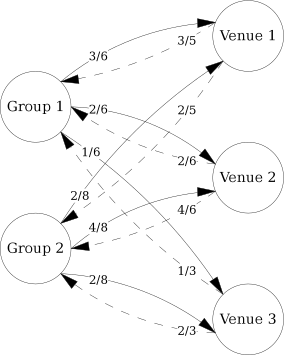
\includegraphics[width=5.2cm]{fig/bhrscore-w3}}
   \caption{Markov chain for an example with two graduate programs and three publication venues.}
   \label{fig:ex1-MC}
\end{figure}

From Figure \ref{fig:ex1-MC}, Group 1 published three papers in Venue 1, two papers in Venue 2, and one paper in Venue 3. Then, the number of publications of Group 1 is six. Venue 1 receives three papers from Group 1, and two papers from Group 2. The fractions of publications from groups to venues and from venues to groups are the edge weights.

Ribas et al.~[\citeyear{ribas17}] have also suggested different possible configurations for the reputation graph. In fact, the sources and collaterals can be any of the three types of entity we consider,  i.e., publication venues, authors, and graduate programs. The targets, however, must always be entities of type venue. That is, we should always use the reputation of venues as the key feature for ranking venues, graduate programs, and individual authors. 

In the next section, we present the initial approaches we adopted to rank academic entities on a per subarea basis and discuss our motivations to modify the standard P-score metric.


%%%%%%%%%%%%%%%%%%%%%
\section{The Encroachment Problem}\label{sec:encroachment}
%%%%%%%%%%%%%%%%%%%%%

Initially, based on the concepts and usability of the standard P-score, we consider a simple hypothesis: to rank academic entities on a per subarea basis, it would be sufficient to use the right reputation sources within a subarea and compute the steady state probabilities of all academic entities. As a result, in theory, the entities with higher P-scores would be the most reputable entities within a subarea. For instance, using as reputation sources the most important venues in Information Retrieval, we would find the most reputable authors, graduate programs, and publication venues in the subarea of IR.

Likewise, the instantiation of P-score in these first experiments, based on one of the possible configurations suggested by Ribas et al.~[\citeyear{ribas2015random}], was as follows: given a pre-selected set of reference venues (or \textit{seeds}) in a given subarea, e.g., conferences or journals, the metric finds the $n$ researchers with the largest volume of publications in these reference venues (for instance, $n$ = 200) and uses them to assemble the Markov network model which also includes all venues in which they published. The steady state probabilities are interpreted as venue weights that distinguish high reputation venues from the others. Thus, these weights can be used to rank venues (by considering these weights as venue scores) and also to rank graduate programs or authors.

However, this approach proves to be inappropriate when considering subareas. The reason is that publication venues possibly cover multiple subareas and thus their reputation needs to be split among their component subareas. One example of such venue is the ACM Conference on Information and Knowledge Management (CIKM). It is a high reputation venue that covers three subareas: Databases (DB), Information Retrieval (IR), and Knowledge Management (KM). If we are interested in the subarea of IR in particular, we need to find a way to discount or weigh down the contributions of CIKM papers that are not on IR. If we do not, we might end with large P-score contributions to a given subarea, such as IR, from papers that are really from another subarea, such as DB. This is what we call the \textit{encroachment problem}. 

We illustrate this problem with an example. Elisa Bertino is a well known and respected researcher who has published over 800 papers. Her interests cover many areas with focus on the fields of Information Security and DB systems. She has papers accepted by CIKM and other venues that also accept papers on IR. Because of that, she appears on the list of authors that publish frequently on IR related venues. And, because of the large number of papers she publishes, her P-score on IR is high, which leads to a high rank of her graduate program at Purdue University on the subarea of IR.

Given that CIKM does not distinguish in its proceedings which papers are on IR, DB or KM, determining whether a given CIKM paper is on IR, for instance, would require examining its text contents. However, P-score is a metric that does not rely on paper contents --- one of its inherent advantages given that it is much simpler to compute than citation-based metrics. Thus, imposing the need to have access to the contents of papers is a constraint we purposely want to avoid. Therefore, we look for a different solution, described in the next section.


%%%%%%%%%%%%%%%%%%%%%
\section{Normalized P-score for Publication Venues}\label{sec:npscore}
%%%%%%%%%%%%%%%%%%%%%

As our primary goal is to perform analysis of academic entities on a per subarea basis, it is crucial to investigate how we could identify suitable publication venues to characterize subareas. 

As originally proposed, P-score venue weights do not allow distinguishing venues in a given subarea, even if we choose as seeds venues that are central to that subarea (i.e., venues which are surely focused on that subarea). This occurs because P-score is a metric strongly correlated to the volume of publications. In other words, venues with high popularity that are related to the seeds --- i.e., have papers written by the authors used as seeds (or references) in the network --- are put in the top positions by the raw P-score.

To avoid this problem, we normalize the venue's P-score by the number of publications in the venue's history. The key idea is to obtain an average of the overall reputation of the venue on a per paper basis. This approach penalizes venues with a large volume of publications but with low P-scores (low reputation according to the seeds) and boosts smaller publication venues with good reputation in a given subarea. Thus, the \textit{normalized P-score} for venue $v$ is defined as: 

\begin{equation}\label{eq:pscore_venue}
    \textit{norm-P-score($v$)} = \frac{\textit{P-score($v$)}}{\textit{number\_of\_publications}(v)}
\end{equation}

Equation (\ref{eq:pscore_venue}) is the starting point for obtaining the ranking of graduate programs on a per subarea basis, as presented in the following section. 

%%%%%%%%%%%%%%%%%%%%%
\section{Weighted P-score for Graduate Programs}\label{sec:wpscore}
%%%%%%%%%%%%%%%%%%%%%

In order to facilitate understanding the modifications we propose for the standard P-score to rank graduate programs by subareas, let us rewrite some equations of standard P-score in a clearer and more concise way than using the whole conceptual framework of reputation flows, focusing on ranking graduate programs itself.

% such as the researchers in Information Retrieval of a given CS graduate program, 
Evaluating a specific graduate program requires weighting the contributions of its members who are responsible for the reputation of the program. Like Ribas et al.~[\citeyear{ribas2015random}], we say that a group's reputation is the sum of the reputation of the venues its members have published in, taken on a per author basis. Moreover, a research publication is usually a combination of efforts by multiple researchers. In consequence, we should normalize the paper's P-score by the number of authors. 
%Let $f(x)$ be any function that measures the reputation of an academic entity $x$. 
Thus:

\begin{equation}\label{eq:pscore_group}
    \textit{P-score($g$)} = \sum_{p \in \theta(g)} \frac{\textit{P-score(venue(p))}}{\textit{number\_of\_authors}(p)}
\end{equation}
where $\theta(g)$ is the set of publications of graduate program $g$ and \textit{venue(p)} is the venue in which paper $p$ was published.
%
In other words, the reputation of a graduate program is based on the papers it published. Each paper has a reputation itself, which is given by the venue where the paper was published. 

{\color{blue}
The research of a graduate program is produced by faculty members, postdoctoral fellows, doctoral students, among others. To determine the correct affiliation of all these graduate program members is a costly task, since that information is often not available and it also dynamically changes (e.g., it is common for graduate students to move from a graduate program to another over the years). However, normally faculty members are responsible for research groups at which postdoctoral fellows and doctoral students work. At some point, the group publishes a paper and its head is typically involved. This allows us to use faculty members as the anchors for the transference of reputation to research groups and, subsequently, to the graduate program these research groups belong. Notice that, in this case, the indication of the faculty member's affiliation is key to estimate reputation for graduate programs. Hence, Equation~(\ref{eq:pscore_group}) may be rewritten as:
}

\begin{equation}\label{eq:pscore_group_author}
    \textit{P-score($g$)} = \sum_{a \in \phi(g)} \sum_{p \in \theta(a)}  \frac{\textit{P-score(venue(p))}}{\textit{number\_of\_authors}(p)}
\end{equation}
where $\phi(g)$ are the researchers associated with graduate program $g$ and $\theta(a)$ are the publications of author $a$. 

Except for the normalization by the number of authors in a paper (which we propose), the Equation~\ref{eq:pscore_group_author} is an alternative way of showing how the standard P-score metric ranks graduate programs, as stated by Equation~\ref{eq:pscore}, in Section~\ref{sec:flows}. However, recap that standard P-score does not provide good ranking of graduate programs on a per subarea basis, due to the encroachment problem described in Section~\ref{sec:encroachment}. 

The solution we propose to the encroachment problem is to examine the main subareas of interest of each researcher and produce weights for the pairs $[researcher, subarea]$. We do so by examining the publications of the researchers on venues that are specific to a single subarea such as SIGIR and SIGMOD, for instance. Our rational is that a researcher that publishes eight SIGIR papers and two SIGMOD papers is focused on IR $80\%$ of the time and on DB 20\% of the time. 
%
In other words, this researcher interest factor on IR is 0.8 and on DB is 0.2. We then use this \textit{subarea interest factor} (hereinafter referred as factor $\gamma$) to weigh the papers of this author in venues that cover multiple subareas, such as CIKM. That is, instead of solving a classification problem (determine the subarea of each CIKM paper), which would require access to paper contents, we propose a ranking solution that ranks CIKM papers on each of its subareas based on their authors' interest factors. Our ranking solution simplifies the implementation and leads to good results, as discussed in Chapter~\ref{sec:results}.

For that, firstly we compute the normalized P-score (Section~\ref{sec:npscore}) to every publication venue based on a subarea $s$ (e.g., Information Retrieval). We claim that the normalized P-score indicates the level of convergence between the publication records of a venue and the specific interests of the subarea. This claim is supported by our results discussed in Chapter~\ref{sec:results}. Then, the set $V_s$ of venues more restricted to that subarea $s$ is defined as:
\begin{equation}
	V_s = \{v \in V\ |\ \textit{norm-P-score($v$)} > \alpha_s\}
\end{equation}
where $V$ is the set of all publication venues, \textit{norm-P-score($v$)} is the normalized P-score for venue $v$ and $\alpha_s$ is a threshold defined by manual inspection of the venues with the highest normalized P-scores for the subarea $s$. 

Once the set $V_{s}$ is defined, we can measure the reputation of authors (and consequently, graduate programs) on a per subarea basis. 
%
With $V_{s}$ being the set of venues closely associated with subarea $s$ and $\theta(a)$ the set of publications of author $a$,  as before, we define:
\begin{equation}\label{eq:author_factor}
    \gamma\text{'}(a,s) = \frac{1}{|\theta(a)|} \sum_{p \in \theta(a)}
    \begin{cases}
         1 & \mbox{if $p \in V_{s}$}\\ 
         0 & \mbox{otherwise} 
    \end{cases}
\end{equation}
where $\gamma\text{'}(a,s)$ is the interest factor of author $a$ in subarea $s$, i.e., a measure of how much the author belongs to that subarea.
% and $\theta(a)$ is the set of publications of author $a$. The results are bound within the interval $[0,1]$, where $1$ means that the author only published in the venues of the subarea (represented by $V_{s}$), and $0$ that she has none publication in the subarea.

Factor $\gamma\text{'}$ quantifies the relation of authors to a given subarea but does not take into account the history of publications by a given author. If an author changes their field of study, we should factor in that the author's relation to the subarea of interest has weakened. We do so by introducing a publication age penalty, as follows:
\begin{equation}\label{eq:author_factor_year}
    \gamma(a,s) = \frac{1}{|\theta(a)|} \sum_{p \in \theta(a)}
    \begin{cases}
      %\varepsilon - \varrho(p) + 1 & \mbox{if $p \in S_{area}$}  \\ 
    %   \frac{1}{\log_2 {(\varepsilon - \varrho(p) + 2)}} & \mbox{if $p \in V_{s}$} \\
      \frac{1}{\log_2 {(y(0) - y(p) + 2)}} & \mbox{if $p \in V_{s}$} \\
      0 & \mbox{otherwise} 
    \end{cases} \\ %y(p) \leq y(0) \\
\end{equation}
where $y(p)$ is the year in which the paper $p$ was published and $y(0)$ is the current year, or the year of the most recent paper in the collection. 

Using the subarea interest factor we can rewrite Equation~(\ref{eq:pscore_group_author}) and present the \textit{weighted P-score} of a graduate program $\textit{g}$ in subarea $\textit{s}$ as:

\begin{equation}\label{eq:group_pscore_author_factor}
    \textit{weighted-P-score($g, s$)} = \sum_{a \in \phi(g)} \gamma(a,s) \times \sum_{p \in \theta(a)} \frac{\textit{P-score(venue(p))}}{\textit{number\_of\_authors}(p)}
\end{equation}

The experimental results of these approaches are presented in Chapter~\ref{sec:results}. In the next section, we describe some considerations on using weighted P-scores to compare research output across different subareas.

\section{Comparing Research in Different Subareas}

Most assessments of this kind consist of analyzing the raw number of publications in each subarea. Likewise, they tend to select few venues that represent the area and then only consider them for the purpose of counting. In here, besides the number of publications, we also consider the reputation of each venue, according to P-score. As shown in Chapter \ref{sec:pscore}, P-score provides encouraging results in ranking academic entities. We aim to show that this metric, when applied to CS graduate programs, allows us to gain valuable insights about the divergences in current publication patterns between different countries.

One final caveat. When we compute P-scores on a per subarea basis, we run a stochastic computation for each subarea. A direct side effect is that P-scores of each subarea, which represent steady state probabilities in a Markov network, are scaled up to sum up to $1$. For comparisons among subareas, this is a problem. In particular, smaller venues might receive disproportionately high relative P-scores due to stochastic scaling in a given subarea. 

Thus, to allow proper comparisons across subareas, we use an artifact we borrow from the computation of Pagerank \citep{page98pagerank}. Inside each subarea, we consider that a fraction of the time, $85\%$ for instance, transitions occur to nodes inside the Markov network for that subarea. The other fraction of the time ($15\%$) transitions occur to nodes in one of the other subareas. The final result is that steady state probabilities of nodes in all subareas must now sum up to 1, which makes them directly comparable. 

%%%%%%%%%%%%%%%%%%%%%
%\section{An Example}
%%%%%%%%%%%%%%%%%%%%%

%%%%%%%%%%%%%%%%%%%%%%%%%%%%%%%%%%%%%%%%%%
\chapter{Experimental Setup}\label{sec:setup}
%%%%%%%%%%%%%%%%%%%%%%%%%%%%%%%%%%%%%%%%%%

In this chapter, we describe the setup supporting our experiments and the key assumptions we have considered on assessing reputation in academia. Specifically, we provide details of the academic dataset we used in this work, the CS subareas considered, the methods we adopted, and previous results used as starting points to our present analysis.

%%%%%%%%%%%%%%%%%%%%%
\section{Dataset}
%%%%%%%%%%%%%%%%%%%%%
% [Characterize DBLP dataset and its enrichment (groups I and csrankings II)]

% # Papers = 2.931.849 | 4.551.362
% # Venues = 5.765
% # Authors = 1.595.771

We compiled a collection of academic publications records extracted from DBLP,\footnote{\url{http://dblp.uni-trier.de}} an online reference for bibliographic information on major CS publications. DBLP data has been used in related studies on CS research communities~\citep{biryukov10,delgado14,hoonlor13,laender2008,wainer13}. 
%
The dataset is publicly available in XML format and contains more than three million publication records from more than 1.5 million authors over the last 50 years, albeit the data before 1970 is rather irregular. Each publication record includes a title, list of authors, year of publication, and publication venue. Publication records do not include the contents of the papers neither information related to citations.

Our collection is actually an extension of the DBLP repository. While it contains all publication venues and authors from DBLP, we have enriched it by adding data regarding graduate programs. To do so, we manually collected data about the top 126  CS graduate programs evaluated in the 2011 assessment conducted by the US National Research Council (NRC).\footnote{\url{http://nap.edu/rdp}}
%
In particular, for each of these graduate programs, we retrieved the list of its members, which was then manually reconciled against the repository.

Despite our efforts, there were still imprecisions related to the affiliation of the authors. To address them, we combined our dataset with the one provided by the \textit{csranking} project,\footnote{\url{http://csrankings.org}} which ranks CS graduate programs based purely on their publications. They do so by collaboratively collecting data on authors, such as their homepage and affiliation. Therefore, we used that data to enhance our repository. Salient statistics on our dataset are shown in Table~\ref{tab:stats}.

\begin{table}[htbp]
\centering
\caption{Salient statistics of the dataset used in our evaluation.}
\label{tab:stats}
\begin{tabular}{l|r}
\toprule
Attribute & Value \\ \hline
Number of Papers         & $2{,}931{,}849$                 \\
Number of Authors        & $1{,}595{,}771$                 \\
Number of Venues         & $5{,}765$                     \\
Number of US Graduate Programs         & $126$                       \\
Avg. number of faculties per US Graduate Program    &    $42.4$                              \\ % 5347 / 126 
Number of BR Graduate Programs          & $25$                        \\
Avg. number of faculties per BR Graduate Program    &    $47.8$                              \\ % 1196 / 25
\bottomrule
\end{tabular}
\end{table}

%%%%%%%%%%%%%%%%%%%%%
\section{Computer Science Subareas}
%%%%%%%%%%%%%%%%%%%%%

There are different ways of defining subareas in CS depending on the institution responsible for the classification. Two notorious classification are given by ACM\footnote{\url{http://acm.org/sigs}} (through its \textit{Special Interest Groups}) and IEEE\footnote{\url{http://computer.org/web/tandc/technical-committees}} (through its \textit{Technical Committees}). 
%
Notice that most of them divide CS into subareas rather distinct. Further, some of these divisions reflect historical decisions that may be less relevant nowadays. For this reason, previous works have attempted to automatically identify such subareas~\citep{wainer13} or use another source of information~\citep{hoonlor13}.

% In this work, we adopt the classification of CS subareas provided by Microsoft Academic 
% Research.\footnote{\url{http://academic.research.microsoft.com}} This classification divides CS in 37 subareas, including relatively new subareas such as Knowledge Management and Natural Languages Processing. The full list of subareas is presented in Table~\ref{tab:subareas}.

A more recent classification is presented by Microsoft Academic Search.\footnote{\url{http://academic.research.microsoft.com}} It divides CS into 37 subareas, including relatively new ones. 
%
For the purpose of this work, we selected 20 subareas from the Microsoft Academic Search classification, as presented in Table~\ref{tab:subareas}. 
{\color{blue}
Along with the list, we present the abbreviation of each subarea, which we will be using from here on. We also show two venues we selected as notorious in each subarea of interest. These venues are important for identifying a group of researchers whose main research topics of interest are likely to be in that subarea --- an essential information for the application of P-score to subareas. However, although the choice of seed venues is an important task, we have observed that any two central venues to a given subarea are sufficient to produce reasonable rankings of publication venues and graduate programs for that subarea.    
}

\begin{table}[h]
%\scriptsize
%\footnotesize
%\normalsize
\small
\centering
\caption{Subareas of Computer Science selected from Microsoft classification. The full names of the publication venues are presented in Appendix~\ref{sec:venues}.}
\label{tab:subareas}
\begin{tabular}{l|c|l} 
\toprule
Subarea                      & Abbreviation & Seed venues          \\ \hline
Algorithms                    & Alg          & SODA, Algorithmica   \\ \hline
Artificial intelligence      & AI           & IJCAI, AI            \\ \hline
Bioinformatics               & Bio          & BIBM, Bioinformatics \\ \hline
Computer graphics            & CG           & SIGGRAPH, TCVG       \\ \hline
Computer networks             & CN           & INFOCOM, TON         \\ \hline
Computer security            & CS           & CCS, TISSEC          \\ \hline
Computer vision              & CV           & CVPR, IJCV           \\ \hline
Data mining                  & DM           & KDD, SIGKDD          \\ \hline
Databases                     & DB           & SIGMOD, TODS         \\ \hline
Distributed computing        & DC           & ICDCS, TPDS          \\ \hline
Human-computer interaction   & HCI          & CHI, TOCHI           \\ \hline
Information Retrieval        & IR           & SIGIR, TOIS          \\ \hline
Machine learning             & ML           & ICML, JMLR           \\ \hline
Natural language processing  & NLP          & EMNLP, COLING        \\ \hline
Operating systems             & OS           & SOSP, SIGOPS         \\ \hline
Parallel computing           & PC           & IPPS, TPDS           \\ \hline
Programming languages         & PL           & PLDI, TOPLAS         \\ \hline
Speech Recognition           & SR           & INTERSPEECH, TCOM    \\ \hline
Theoretical computer science & TCS          & STOC, SIAMCOMP       \\ \hline
World Wide Web               & WWW          & WWW, WS              \\ 
\bottomrule
\end{tabular}
\end{table}

{\color{blue}
% We avoided using all 37 subareas because we found some of them difficult to characterize. 
%
While our subset of 20 CS subareas is not perfect or exhaustive, it is detailed enough to allow gaining insights into the scene of research in CS in Brazil, which would not be possible to obtain otherwise. In Appendix~\ref{sec:cs-subareas}, we present other classifications of CS subareas, according to reliable sources.

An alternative configuration of P-score consists in using a set of researchers with high reputation as seed, instead of publication venues. In particular, on a per subarea basis, one can identify the most reputable researchers in a given subarea, use them as seeds of reputation in P-score, and subsquently finds the most important venues in that subarea. To automatically identify these most reputable researchers, we made experiments using clustering techniques on a graph of coauthorships, where the nodes were individual researchers and the edges represented coautorships between them, as discussed in Appendix~\ref{sec:clustering}. Then, for each cluster in the subarea, we selected the top $n$ most representative researchers as reputation seeds. This methodology produced similar results when compared to the use of venues as seeds and can be improved in the future by enriching the graph of coauthorships with more information about each researcher, such as academic productivity and centrality metrics. Moreover, clustering methods on academic networks can also help in an automatic identification of the current subareas in the broad area of CS.
}

%%%%%%%%%%%%%%%%%%%%%
\section{Venues Ground-Truth}\label{sec:venue-ground-truth}
%%%%%%%%%%%%%%%%%%%%%

To evaluate the effectiveness of normalized P-scores as defined by Equation (\ref{eq:pscore_venue}) on the task of finding venues in a subarea, we considered as ground-truth the opinion of experts. Specifically, we asked reputable CS researchers and their graduate students, working on subareas of IR, DB and Data Mining (DM) to assess the relevance of venues (included in a pre-selected list) to their subareas. This list consists of the venues at the top 50 positions in the P-score ranking when we use as seeds two publication venues only: a journal and a conference closely associated with that subarea. For examples of seeds, see Table~\ref{tab:seeds}.

\begin{table}[htbp]
\centering
\caption{Seeds of publication venues for the P-score ranking used in this work.}
\label{tab:seeds}
\begin{tabular}{l|ccc}
\toprule
                                   & \multicolumn{3}{c}{Subareas}                                                            \\ \hline
\multicolumn{1}{c|}{Type of venue} & \multicolumn{1}{c|}{Databases} & \multicolumn{1}{c|}{Data Mining} & Information Retrieval \\ \hline
\multicolumn{1}{l|}{Conference}    & \multicolumn{1}{c|}{SIGMOD}   & \multicolumn{1}{c|}{KDD}         & SIGIR                 \\ \hline
\multicolumn{1}{l|}{Journal}       & \multicolumn{1}{c|}{TODS}     & \multicolumn{1}{c|}{SIGKDD}      & TOIS                 \\
\bottomrule
\end{tabular}
\end{table}

We thus focused on the CS subareas of DB, DM, and IR. For each subarea, three experts have classified each of the 50 venues of the pre-selected list into one, two or three subareas chosen among the 37 subareas listed in Table~\ref{tab:subareas}. To reconcile the multiple classifications, we used a majority criterion: if a publication venue $v$ was associated with a subarea $s$ at least twice, $s$ was considered as one of the subareas of $v$. Hereafter, we will refer to the full lists of publication venues and their subareas as our \textit{venues ground-truth}.

% As a result, that allows us to perform a precision-recall analysis of different approaches in finding  the  given a subarea, as shown in Figure~\ref{fig:norm-pscore-curves}. For the evaluation, we have considered only the same 50 publication venues already classified by the experts. For this reason, all strategies reach the maximum recall (100\%) at the end of each curve. We used the H-index metric and the standard P-score as competitors for the normalized P-score. For the both metrics based on the P-score, we have chosen the same initial seeds of reputation, as shown in the Table~\ref{tab:seeds}.

% other filterings
% Venues: min-pub=100, live-in:2012

%%%%%%%%%%%%%%%%%%%%%
%\section{Evaluation Methodology}
%%%%%%%%%%%%%%%%%%%%%
%\subsection*{Ranking Venues}\label{sec:eval-venues}
%Competitors: 
%
%H-index
%
%Standard P-score
%
%H-indices were obtained from Google Scholar.

%%%%%%%%%%%%%%%%%%%%%%%%%%%%%%%%%%%%%%%%%%
\chapter{Experimental Results}\label{sec:results}
%%%%%%%%%%%%%%%%%%%%%%%%%%%%%%%%%%%%%%%%%%

In this chapter, we discuss the results of ranking publication venues and graduate programs in CS on the three subareas we selected: Information Retrieval, Databases, and Data Mining. In particular, for the ranking of graduate programs, our results are restricted to the 126 US graduate programs considered by NRC in 2011.

% In particular, in this chapter we aim to answer the research question Q1) \textit{How to quantify the reputation of publication venues and graduate programs on a per subarea basis?}. In Sections \ref{sec:results-us} and \ref{sec:results-br} we intend to answer the research question Q2) \textit{How does the reputation of Brazilian and US graduate programs in CS vary per subarea?}. Lastly, in Section \ref{sec:comparison}, we discuss question Q3) \textit{Are there differences between the current research directions in CS of the top Brazilian and US graduate programs?}

%%%%%%%%%%%%%%%%%%%%%
\section{Ranking Venues}\label{sec:results-venues}
%%%%%%%%%%%%%%%%%%%%%

Using the normalized P-score (norm-P-score) presented in Section \ref{sec:npscore}, we were able to better discriminate publication venues of a given CS subarea from venues of other subareas. Figure~\ref{fig:norm-pscore-curves-ir} presents the precision-recall curve obtained by norm-P-score in the task of ranking publication venues in Information Retrieval, in light of the results produced using two other methods, namely H-index and standard P-score.
%
To produce the precision-recall curves, we use as ground-truth a venue classification done by experts in each subarea, see Section~\ref{sec:venue-ground-truth}. We reproduced the same experimental methodology for ranking venues in the subareas of Databases and Data Mining. The precision-recall curves are shown in Figure \ref{fig:norm-pscore-curves-db-dm}.

\begin{figure}[htbp]
    \centering
    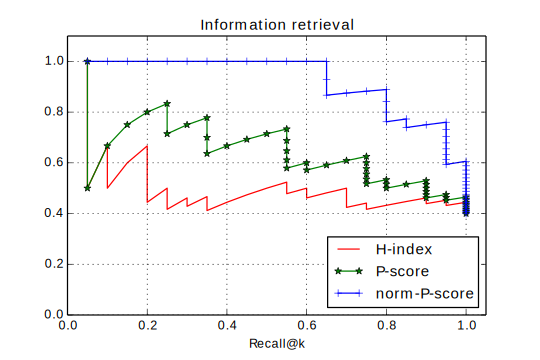
\includegraphics[width=0.8\linewidth]{fig/ir-prec-recall.eps}
    \caption{Precision-Recall curves of H-index, P-score and normalized P-score for the subarea of Information Retrieval.}
    \label{fig:norm-pscore-curves-ir}
\end{figure}

\begin{figure}[htbp]
    \centering
    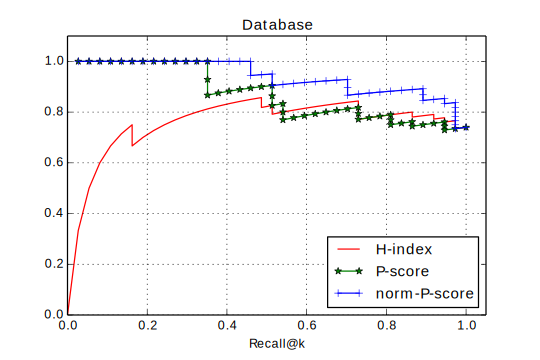
\includegraphics[width=0.8\linewidth]{fig/db-prec-recall.eps}
    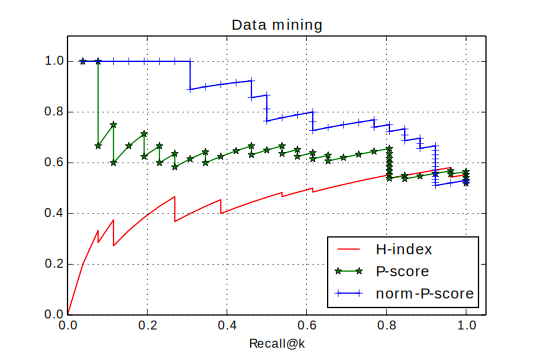
\includegraphics[width=0.8\linewidth]{fig/dm-prec-recall.eps}
    \caption{Precision-Recall curves of H-index, P-score and normalized P-score for the subareas of Databases and Data Mining.}
    \label{fig:norm-pscore-curves-db-dm}
\end{figure}

As it is clear from Figures \ref{fig:norm-pscore-curves-ir} and \ref{fig:norm-pscore-curves-db-dm}, normalized P-scores allow identifying the correct venues consistently better than H-indices and standard P-scores. Furthermore, for all the three subareas, the normalized P-scores yield maximum precision ($100\%$) for the initial $30\%$ of recall. This means that the first 15 venues in the normalized P-score ranking adopted in Figure \ref{fig:norm-pscore-curves-ir} are strongly related to IR, according to the assessments of specialists.

To further illustrate, Table~\ref{tab:ir-venues} shows the top 20 publication venues for the subarea of IR, produced by P-scores and normalized P-scores when we consider SIGIR and TOIS as seed venues. Also, a final ranking of IR venues is computed by re-ranking the venues --- previously filtered by normalized P-score --- according to their standard P-scores.

On the one hand, the standard P-score metric places venues such as the International World Wide Web Conferences (WWW) and the International Conference on Multimedia (MM), among the top 10 positions. These two conferences cover topics of the IR subarea, but indeed have a larger scope than IR only. 
%
On the other hand, such conferences do not appear in the normalized P-score ranking, even among the top 20 positions on the ranking. Besides, in the normalized P-score ranking, venues mainly focused on IR venues such as the International Conference on the Theory of Information Retrieval (ICTIR) and Transactions on Information Systems (TOIS) appear among the top 20 publication venues. This power of discrimination of the normalized P-score is important to allow selecting venues that better represent the subarea of IR.

Similar results can be found in Tables~\ref{tab:db-venues} and~\ref{tab:dm-venues}, for the subareas of DB and DM, respectively. In DB, venues with a large scope such as WWW and International Conference on Data Mining (ICDM), although with high standard P-scores, are not selected among the top 20 venues according to the normalized P-score metric. In DM, venues such as the AAAI Conference on Artificial Intelligence and the Conference on Neural Information Processing Systems (NIPS), clearly not mainly focused on DM, are also filtered by the normalized P-score. In summary, for both subareas (DB and DM), the final ranking contains several publication venues highly focused on each subarea.

%\raisebox{-\totalheight}{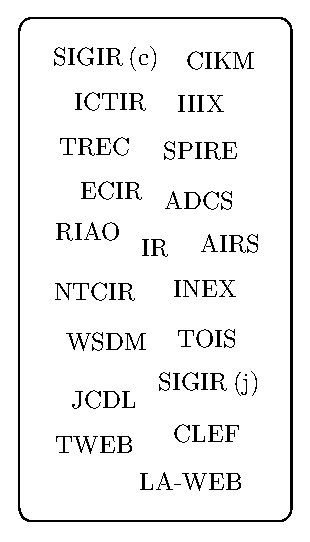
\includegraphics[width=0.3\textwidth]{fig/ir-norm-venues-blob.eps}} 

\begin{table}[htbp]
\centering
\caption{Top 20 venues in Information Retrieval using (i) standard P-score, (ii) the set of venues selected by the normalized P-score, and (iii) re-ranking the set of venues obtained in (ii) according to their P-scores. The suffixes (c) and (j) are used to differentiate conferences and journals with the same name. The full names of the publication venues are presented in Appendix~\ref{sec:venues}.}
\label{tab:ir-venues}
%\resizebox{\columnwidth}{!}{%
\begin{tabular}{rc}
\toprule
\#		&	Standard P-score \\ 
\midrule
1		&	SIGIR (c) \\
2		&	CIKM		\\
3		&	TREC	\\	
4		&	ECIR		\\
5		&	CLEF		\\
6		&	WWW	\\		
7		&	JASIS	\\	
8		&	IPM		\\	
9		&	SIGIR (j) \\
10		&	MM	\\		
11		&	JCDL		\\
12		&	TOIS		\\
13		&	IR			\\
14		&	WSDM	\\
15		&	NTCIR	\\
16		&	KDD		\\
17		&	TKDE	\\
18		&	ACL		\\
19		&	ICDM		\\
20		&	SPIRE	\\
\bottomrule
\end{tabular} \ \ 
\begin{tabular}{c}
\toprule
norm-P-score \\ 
\midrule
%\vspace{-30px}
\multirow{20}{*}{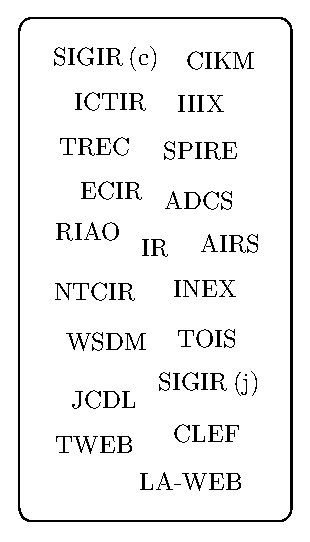
\includegraphics{fig/ir-norm-venues-blob.eps}} \\ %[width=0.2\linewidth]
\\
\\
\\
\\
\\
\\
\\
\\
\\
\\
\\
\\
\\
\\
\\
\\
\\
\\
\\
\bottomrule
\end{tabular} \ \
\begin{tabular}{rc}
\toprule
\#		&	Final Ranking \\ 
\midrule
1		&	SIGIR (c)	\\
2		&	CIKM		\\
3		&	TREC		\\
4		&	ECIR		\\
5		&	CLEF		\\
6		&	SIGIR (j)	\\
7		&	JCDL		\\
8		&	TOIS		\\
9		&	IR			\\
10		&	WSDM		\\
11		&	NTCIR		\\
12		&	SPIRE		\\
13		&	AIRS		\\
14		&	RIAO		\\
15		&	INEX		\\
16		&	IIIX		\\
17		&	ICTIR		\\
18		&	ADCS		\\
19		&	LA-WEB		\\
20		&	TWEB		\\
\bottomrule
\end{tabular}
\end{table}

\begin{table}[htbp]
\centering
\caption{Top 20 venues in Databases, using (i) standard P-score, (ii) the set of venues selected by the normalized P-score, and (iii) re-ranking the set of venues obtained in (ii) according to their P-scores. The suffixes (c) and (j) are used to differentiate conferences and journals with the same name.  The full names of the publication venues are presented in Appendix~\ref{sec:venues}.}
\label{tab:db-venues}
%\resizebox{\columnwidth}{!}{%
\begin{tabular}{rc}
\toprule
\#		&	Standard P-score \\ 
\midrule
1		&		SIGMOD (c)	\\
2		&		ICDE		\\
3		&		VLDB (c)	\\
4		&		PVLDB		\\
5		&		TKDE		\\
6		&		DEBU		\\
7		&		SIGMOD (j)	\\
8		&		EDBT		\\
9		&		CIKM		\\
10		&		PODS		\\
11		&		TODS		\\
12		&		KDD			\\
13		&		VLDB (j)	\\
14		&		WWW			\\
15		&		ICDM		\\
16		&		DASFAA		\\
17		&		SSDBM		\\
18		&		IS			\\
19		&		ICDT		\\
20		&		CIDR		\\
\bottomrule
\end{tabular} \ \ 
\begin{tabular}{c}
\toprule
norm-P-score \\ 
\midrule
%\vspace{-30px}
\multirow{20}{*}{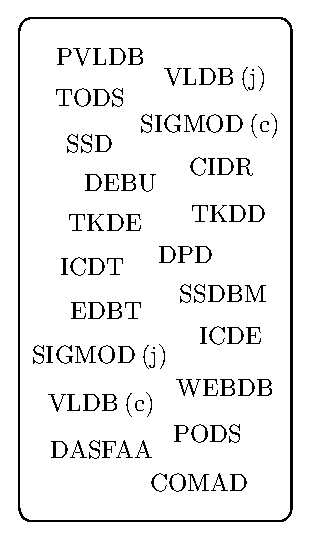
\includegraphics{fig/db-norm-venues-blob.eps}} \\ %[width=0.2\linewidth]
\\
\\
\\
\\
\\
\\
\\
\\
\\
\\
\\
\\
\\
\\
\\
\\
\\
\\
\\
\bottomrule
\end{tabular} \ \
\begin{tabular}{rc}
\toprule
\#		&	Final Ranking \\ 
\midrule
1		&		SIGMOD (c)	\\
2		&		ICDE		\\
3		&		VLDB (c)	\\
4		&		PVLDB		\\
5		&		TKDE		\\
6		&		DEBU		\\
7		&		SIGMOD (j)	\\
8		&		EDBT		\\
9		&		PODS		\\
10		&		TODS		\\
11		&		VLDB (j)	\\
12		&		DASFAA		\\
13		&		SSDBM		\\
14		&		ICDT		\\
15		&		CIDR		\\
16		&		WEBDB		\\
17		&		SSD			\\
18		&		DPD			\\
19		&		COMAD		\\
20		&		TKDD		\\
\bottomrule
\end{tabular}
\end{table}

\begin{table}[htbp]
\centering
\caption{Top 20 venues in Data Mining, using (i) standard P-score, (ii) the set of venues selected by the normalized P-score, and (iii) re-ranking the set of venues obtained in (ii) according to their P-scores. The suffixes (c) and (j) are used to differentiate conferences and journals with the same name. The full names of the publication venues are presented in Appendix~\ref{sec:venues}.}
\label{tab:dm-venues}
%\resizebox{\columnwidth}{!}{%
\begin{tabular}{rc}
\toprule
\#		&	Standard P-score \\ 
\midrule
1		&		KDD			\\
2		&		ICDM		\\
3		&		CIKM		\\
4		&		ICDE		\\
5		&		ICML		\\
6		&		SDM			\\
7		&		TKDE		\\
8		&		WWW			\\
9		&		SIGMOD		\\
10		&		AAAI		\\
11		&		PKDD		\\
12		&		NIPS		\\
13		&		PAKDD		\\
14		&		VLDB (c)	\\
15		&		SIGIR		\\
16		&		SIGKDD		\\
17		&		DATAMINE	\\
18		&		KAIS		\\
19		&		JMLR		\\
20		&		PVLDB		\\
\bottomrule
\end{tabular} \ \ 
\begin{tabular}{c}
\toprule
norm-P-score \\ 
\midrule
%\vspace{-30px}
\multirow{20}{*}{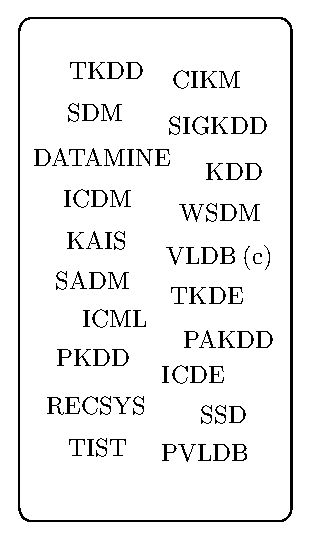
\includegraphics{fig/dm-norm-venues-blob.eps}} \\ %[width=0.2\linewidth]
\\
\\
\\
\\
\\
\\
\\
\\
\\
\\
\\
\\
\\
\\
\\
\\
\\
\\
\\
\bottomrule
\end{tabular} \ \
\begin{tabular}{rc}
\toprule
\#		&	Final Ranking \\ 
\midrule
1		&		KDD			\\
2		&		ICDM		\\
3		&		CIKM		\\
4		&		ICDE		\\
5		&		ICML		\\
6		&		SDM			\\
7		&		TKDE		\\
8		&		PKDD		\\
9		&		PAKDD		\\
10		&		SIGKDD		\\
11		&		DATAMINE	\\
12		&		KAIS		\\
13		&		PVLDB		\\
14		&		WSDM		\\
15		&		TKDD		\\
16		&		VLDB (c)	\\
17		&		RECSYS		\\
18		&		TIST		\\
19		&		SSD			\\
20		&		SADM		\\
\bottomrule
\end{tabular}
\end{table}

It is noteworthy to mention that the normalized P-score ranking of venues should not be interpreted as an impact or productivity ranking. We only use this output to define the most representative venues of a subarea, in a semi-automatic fashion. For this reason, in Tables~\ref{tab:ir-venues},~\ref{tab:db-venues}, and~\ref{tab:dm-venues}, we present the results obtained by normalized P-scores as sets of venues instead of usual rankings of venues.

Afterward, using this ranking of publication venues as a starting point, we can improve rankings of graduate programs in CS by considering a per subarea basis. Our results in ranking graduate programs are discussed in the next section.

%%%%%%%%%%%%%%%%%%%%%
\section{Ranking US Graduate Programs by Subarea}\label{sec:results-us}
%%%%%%%%%%%%%%%%%%%%%

For this section, we are interested in the distribution of publications in the CS subareas of graduate programs across US. More specifically, we want to understand which subareas receive more attention by the top graduate programs in US. 

%P-score provides good rankings of venues~\citep{ribas2015random}, however, rankings of graduate programs using standard P-score are disrupted by the encroachment discussed in Section~\ref{sec:encroachment}. In a broad area as CS, one should consider each subarea separately rather than evaluating the whole area, since they are not the same. Therefore, we propose to rank US graduate programs considering subareas. 
As in Section \ref{sec:results-venues}, we consider the same three CS subareas: IR, DB, and DM.

%%%%%%%%%%
\subsection*{Information Retrieval, Databases, and Data Mining}
%%%%%%%%%%
%% IR 
Table~\ref{tab:top10-ir-pscore} presents a ranking of US universities based on standard P-scores for the IR subarea. The values presented are normalized to $1$ as follows:
\begin{equation}\label{eq:norm-values}
    \overline{P}(g,s) = \frac{P(g,s)}{max(P(g,s))}
\end{equation}
where $\overline{P}(g,s)$ is the normalized score of graduate program $g$ in subarea $s$, $P(g,s)$ is the score and $max(P(g,s))$ is the highest score of the ranking. We apply Equation~\ref{eq:norm-values} to either standard and weighted P-scores.

\begin{table}[htbp]
\centering
\caption{Ranking of the top 10 US Universities on Information Retrieval, based on standard P-scores.}
\label{tab:top10-ir-pscore}
\begin{tabular}{rlr}
    \toprule
    \# & University                                 & \multicolumn{1}{c}{P-score} \\
    \midrule
    1  & Carnegie Mellon University                 & $1$            \\
    2  & University of Massachusetts Amherst        & $0.8082$ \\
    3  & University of Illinois at Urbana-Champaign & $0.6735$ \\
    4  & University of Southern California          & $0.4541$ \\
    5  & Georgia Institute of Technology            & $0.4341$ \\
    6  & Stanford University                        & $0.3493$ \\
    7  & University of Illinois at Chicago          & $0.3409$ \\
    8  & Cornell University                         & $0.3344$ \\
    9  & University of California-Berkeley          & $0.3337$ \\
    10 & Purdue University                          & $0.3120$ \\
    \bottomrule
\end{tabular}
\end{table}

The University of Massachusetts Amherst has the premier IR research group in the US and, thus, the fact that it was not in first place in the rank was surprising to us. This led to an in-depth analysis of the ranking and the consequent understanding of the encroachment problem, as discussed in Section~\ref{sec:encroachment}. 
%
Table~\ref{tab:top10-ir} presents the top 10 graduate programs for the IR subarea using our proposed approach of the weighted P-score, according to Equation~(\ref{eq:group_pscore_author_factor}), instead. We observe that the University of Southern California, the Georgia Institute of Technology, Stanford University and the University of California at Berkeley are no longer among the top 10 graduate programs. This seems appropriate given these universities are not active on research in IR.

\begin{table}[htbp]
\centering
\caption{Ranking of the top 10 US Universities on Information Retrieval, using the weighted P-score (Equation~\ref{eq:group_pscore_author_factor}).}
\label{tab:top10-ir}
\begin{tabular}{rlr}
    \toprule
    \# & University                                 & \multicolumn{1}{c}{weighted-P-score} \\
    \midrule
    1  & University of Massachusetts Amherst        & $1$                         \\
    2  & University of Illinois at Urbana-Champaign & $0.4830$                    \\
    3  & Carnegie Mellon University                 & $0.4625$                    \\
    4  & University of Delaware                     & $0.2452$                    \\
    5  & Purdue University                          & $0.2276$                    \\
    6  & Northeastern University                    & $0.1633$                    \\
    7  & Lehigh University                          & $0.0964$                    \\
    8  & Cornell University                         & $0.0552$                    \\
    9  & University of Iowa                         & $0.0494$                    \\
    10 & University of Illinois at Chicago          & $0.0477$                    \\
    \bottomrule
\end{tabular}
\end{table}

To better understand the results in Table~\ref{tab:top10-ir}, we produced a list of the top 20 researchers on IR. Table~\ref{tab:top-authors} shows their affiliations. As we observe, our top 10 graduate programs for the IR subarea are those whose researchers are also among the top 20 authors on IR in the US. In particular, the top 3 groups have each one 2 or more researchers among the top 20. 
%
We also manually examined our ranking of authors to observe that the top authors showed in Table~\ref{tab:top-authors} had more publications in venues strongly related to the subarea. Hence, the ranking of graduate programs can be justified by the ranking of authors. 
%
We repeated this process to the DB and DM subareas. Tables~\ref{tab:top10-db} and~\ref{tab:top10-dm} present the top 10 graduate programs on DB and DM, when we use the weighted P-scores produced by Equation~(\ref{eq:group_pscore_author_factor}).

\begin{table}[htbp]
\centering
\caption{Ranking of the top 20 US researchers' universities on Information Retrieval, using Equation~(\ref{eq:group_pscore_author_factor}).}
\label{tab:top-authors}
\begin{tabular}{rl}
    \toprule
    \# & Authors' universities \\
    \midrule
    1  & University of Massachusetts Amherst \#1        \\
    2  & University of Massachusetts Amherst \#2        \\
    3  & Carnegie Mellon University \#1                 \\
    4  & University of Illinois at Urbana-Champaign \#1 \\
    5  & Purdue University                            \\
    6  & University of Delaware                       \\
    7  & Northeastern University                      \\
    8  & University of Illinois at Urbana-Champaign \#2 \\
    9  & Lehigh University                            \\
    10 & Carnegie Mellon University \#2                 \\
    11 & University of Iowa                           \\
    12 & University of Illinois at Chicago            \\
    13 & Georgia Institute of Technology              \\
    14 & University of Virginia                       \\
    15 & Carnegie Mellon University \#3                 \\
    16 & Texas A\&M University                        \\
    17 & Cornell University                           \\
    18 & University of Michigan                       \\
    19 & University of Massachusetts Amherst \#3        \\
    20 & New York University                          \\
\bottomrule
\end{tabular}
\end{table}

\begin{table}[htbp]
\centering
\caption{Ranking of the top 10 US Universities on Databases, using the weighted P-score (Equation~(\ref{eq:group_pscore_author_factor})).}
\label{tab:top10-db}
\begin{tabular}{rlr}
    \toprule
    \# & University                                 & \multicolumn{1}{c}{weighted-P-score} \\
    \midrule
    1    & University of Wisconsin-Madison                & $1$        \\
    2    & Stanford University                            & $0.6570$    \\
    3    & University of Illinois at Urbana-Champaign    & $0.5687$    \\
    4    & Massachusetts Institute of Technology            & $0.4975$    \\
    5    & Duke University                                & $0.4616$    \\
    6    & University of Massachusetts Amherst            & $0.4243$    \\
    7    & University of Michigan                        & $0.4195$    \\
    8    & University of California-Irvine                & $0.4120$    \\
    9    & University of Maryland-College Park            & $0.4101$    \\
    10    & University of California-Santa Cruz            & $0.3982$    \\
    \bottomrule
\end{tabular}
\end{table}

\begin{table}[htbp]
\centering
\caption{Ranking of the top 10 US Universities on Data Mining, using the weighted P-score (Equation~(\ref{eq:group_pscore_author_factor})).}
\label{tab:top10-dm}
\begin{tabular}{rlr}
    \toprule
    \# & University                                 & \multicolumn{1}{c}{weighted-P-score} \\
    \midrule
    1    & University of Illinois at Chicago                & $1$        \\
    2    & Carnegie Mellon University                    & $0.6857$    \\
    3    & University of Illinois at Urbana-Champaign    & $0.6344$    \\
    4    & University of Minnesota                        & $0.5350$    \\
    5    & Arizona State University                        & $0.4276$    \\
    6    & University of California-Riverside            & $0.4212$    \\
    7    & Georgia Institute of Technology                & $0.3955$    \\
    8    & University of Michigan                        & $0.3275$    \\
    9    & Rensselaer Polytechnic Institute                & $0.2761$    \\
    10    & University of California-Davis                & $0.2593$    \\
    \bottomrule
\end{tabular}
\end{table}

Our analysis on a per subarea basis uncovers venues and graduate programs that are not always thought of as being of high excellence. But, once one considers their track records on a specific subarea, it is clear that they are quite productive. That is, analyzing graduate programs on a per subarea basis yields insights that are hidden when we apply global metrics of productivity to a broad area as CS.

%%%%%%%%%%
\subsection*{US Research Overview}
%%%%%%%%%%

For the results presented here, we used the weighted P-score (Equation~\ref{eq:group_pscore_author_factor}) to rank graduate programs in the 20 subareas selected. To do so, we first got the P-score for each subarea, where we used as seeds the venues in Table~\ref{tab:subareas}. After that, normalized P-scores allowed us to select the top venues that more adequately represent each subarea. Following, we used them to compute the weighted P-score for each graduate program in each subarea. Finally, we selected the top 20 graduate programs in US, for each subarea. Figure \ref{fig:us-research} presents the results we obtained.

Figure~\ref{fig:us-research} presents our experiments considering only CS graduate programs in the US. It shows the cumulative weighted P-score for the top 20 CS graduate programs in each of the 20 subareas. We observe that Computer Vision is the subarea with highest cumulative weighted P-score, followed by Databases, Theoretical Computer Science, and Machine Learning.

\begin{figure}[tb] %htbp
    \centering
    \includegraphics[width=0.9\linewidth]{fig/char_us_research_new.eps}
    \caption{Distribution of cumulative weighted P-scores for the top 20 US graduate programs on a per subarea basis.}
    \label{fig:us-research}
\end{figure}

Computer Vision attracts a lot of attention and interest nowadays because it is present in some of the most cutting-edge technologies, such as autonomous vehicles which demand a massive amount of computer vision processing. On the other hand, Theoretical CS (TCS) may appear a bit surprising. It is an area where publishing is slightly more difficult, especially because it often demands time, e.g., to prove theorems, and faculty usually advise fewer students and are thus likely to produce fewer papers~\citep{wainer13}. Despite this, our experiments showed TCS in third place. When inspecting the number of publications, we noticed that they have fewer than others, indeed. However, P-scores for venues in TCS were rather significant, indicating that the subarea has various venues of high reputation.

Another surprising subarea observed from Figure~\ref{fig:us-research} is Machine Learning (ML). While it is a remarkable growing field of study, we observed that P-scores of ML venues were not well distributed. One problem that we noticed is that ML is extremely multidisciplinary. Therefore, several venues with notorious work for the ML subarea also contain important publications for other subareas, i.e., they are not venues dedicated exclusively to ML. Moreover, many subareas include Machine Learning related research (a good example is Computer Vision).

%This becomes a problem because it is harder to find pure venues dedicated exclusively to Machine Learning.

Databases and Computer Networks are also well positioned in our experiment. They are more traditional fields of study (TCS as well) and have a considerable amount of work developed in the past. 

%%%%%%%%%%%%%%%%%%%%%
\section{Ranking BR Graduate Programs by Subarea}\label{sec:results-br}
%%%%%%%%%%%%%%%%%%%%%

We apply the same methodology of Section~\ref{sec:results-us} for assessing the reputation of CS graduate programs in Brazil. Figure~\ref{fig:br-research} presents our findings. It shows the cumulative weighted P-score for the top 20 CS graduate programs in each of the 20 subareas. According to our results, Parallel Computing is the subarea with the highest cumulative weighted P-score (considerably higher than the others), followed by Information Retrieval and Computer Graphics.

\begin{figure}[tb]
    \centering    
    \includegraphics[width=0.9\linewidth]{fig/char_br_research_new.eps}
    \caption{Distribution of cumulative weighted P-scores for the top 20 BR graduate programs per subarea.}
    \label{fig:br-research}
\end{figure}

We also observe that P-scores in Brazil are almost two orders of magnitude smaller than those in the US. Thus, while the volume of publications in Brazil is relatively high \citep{laender2008}, their impact in terms of exposure in high reputation venues is rather modest. 

Computer Science production in Brazil is considerably uneven. Many subareas have extremely low scores, in some of them, the score is almost inexistent.
%
Thus, while there are researchers in Brazil working on all subareas, the number of papers published in reputable venues in several subareas is rather small. 
%
In contrast, we noted that in some CS subareas there are Brazilian graduate programs as reputable as top US graduate programs. For instance, Figure \ref{fig:ranking-ir} shows the top 20 graduate programs in Information Retrieval, according to the weighted P-score. We observe two Brazilian graduate programs among these programs. This is noteworthy, given this kind of finding would not be possible without considering a per subarea analysis.

\begin{figure}[htbp]
    %\centering
     \includegraphics[width=\linewidth]{fig/ir_groups.eps}
    \caption{Top 20 Graduate Programs for the Information Retrieval subarea, according to weighted P-score, considering US and BR graduate programs, using logarithmic-scale.}
    \label{fig:ranking-ir}
\end{figure}

%%%%%%%%%%%%%%%%%%%%%
\section{Comparing BR and US Research in CS}\label{sec:comparison}
%%%%%%%%%%%%%%%%%%%%%

In Figure~\ref{fig:br-research-us-order} we reorder the results presented in Figure~\ref{fig:br-research} according to the same order of subareas in the US graduate programs in Figure~\ref{fig:us-research}, with the purpose of comparing the CS research scenario in Brazil and in US.

\begin{figure}[tb]
    \centering
    \includegraphics[width=0.9\linewidth]{fig/char_br_us_research_new.eps}
    \caption{Distribution of cumulative weighted P-scores for the top 20 BR graduate programs per subarea, in the same subarea order of Figure \ref{fig:us-research}.}
    \label{fig:br-research-us-order}
\end{figure}

In Brazil, Parallel Computing and Information Retrieval are the subareas with the highest scores, while in the US the two subareas of greatest interest are Computer Vision and Databases. 
%
{\color{blue} 
We also observe that the five subareas of greatest interest in Brazil are very distinct from those of greatest interest in US. If we consider that the top US graduate programs are among the best programs world widely and also that their research directions are the key subareas in CS nowadays, this experiment suggests that academic research in Brazil is not shifting its focus of attention as fast as it happens in the US. 

A possible explanation for this result may be the resistance by Brazilian CS researchers to move from their original subareas of study to new ones, or include modern subareas in their research interests, over the decades. This behavior can be motivated by personal reasons but also by a lack of support from government officials and funding agencies. With the increasing interest of solid companies in high advanced technologies and capable human resources, public-private partnerships can stimulate research of excellence in these modern subareas, what can direct benefit graduate programs in the next years.  

Overall, this type of analysis can be important for those who need to decide how to allocate limited research funds. Although it is known that the volume of US scientific publications in CS is significantly superior to the volume of Brazilian CS research, this comparison shows that the CS subareas in which each country has major scientific impact are basically disjoint. 
}

%%%%%%%%%%%%%%%%%%%%%%%%%%%%%%%%%%%%%%%%%%
\chapter{Conclusions and Future Work}\label{sec:conclusions}
%%%%%%%%%%%%%%%%%%%%%%%%%%%%%%%%%%%%%%%%%%

In this dissertation, our first research question was: \textit{``How to quantify the reputation of publication venues and graduate programs on a per subarea basis?''} We presented experiments suggesting that metrics that only capture broad features of a subarea such as the volume of publications, citations or general reputation (standard P-score included) are not sufficient to produce reasonable rankings on a per subarea basis. In particular, we demonstrated that solving the venues encroachment problem allows us to improve the ranking of graduate programs in a given subarea. We showed a simple but effective strategy to increase or decrease the contribution of an author to the overall reputation of her graduate program in a given subarea, based on the author's relation to that subarea. 

Our second research question was: \textit{``How does the reputation of Brazilian and US graduate programs in CS vary per subarea?''} We showed that the identification of the most reputable publication venues and graduate programs in Computer Science depends on the subarea considered to the task. Specifically, both the most suitable venues as the rankings of Brazilian and US graduate programs vary on a per subarea basis, considering the subareas of Information Retrieval, Databases and Data Mining. Besides, we described how to modify the P-score metric to find the core venues of a subarea in a semi-automatic fashion and, subsequently, how to rank graduate programs using this information, obtaining the top graduate programs of a given subarea.

Our third research question was: \textit{``Are there differences between the current research directions in CS of the top Brazilian and US graduate programs?''} We showed that, in terms of reputation, the current research of the top graduate programs in Brazil and US differ considerably. It is known that the volume of US scientific publications in CS is significantly superior to the volume of Brazilian CS research. However, this work shows that the CS subareas in which each country has major scientific impact are basically disjoint. 
Moreover, the large distance between the reputation scores of Brazil and US programs emphasizes the focus of US researchers on publishing in the most reputable conferences and journals within their subareas. 

% In this paper, our first research question was: \textit{``How does the reputation of Brazilian graduate programs in CS vary per subarea?''} We showed that the definition of the most reputable Brazilian graduate programs in CS depends on the subarea we take into account. For instance, in Information Retrieval, there is a significant distance between the top 3 (?) programs and the others. Similar behavior could be observed in the subareas of Databases and Computer Networks. Moreover, we showed that Brazilian graduate programs are concentrated in subareas such as  Computer Graphics, Information Retrieval, and Parallel Computing. This kind of information provides insights to government funding agencies, university officials, department chairs on how to allocate research fundings. 

% Rephrase / Introduction of conclusions?
%Our intent is to show that reputation flows can be used to gain insight into the productivity of individual researchers and of graduate programs, not that a ranking based on a single metric should be taken at face value. Instead, the decision on how to classify or rank individual researchers and graduate programs can only be made by committees composed of human specialists. However, even under this light, committees of specialists need data and metrics that can be used to support their decisions.
%
%Additionally, the framework of reputation flows provides a complementary view on the reputation of academic entities which allows implementation of new features, such as notification alerts on new venues with rising reputation, as discussed in Ribas et al. [2017].
%%

For future work, we plan to use academic data of graduate programs from other regions of the world, such as Europe and Asia, and, thereupon, characterize the distribution of the most reputable graduate programs in CS worldwide, on a per subarea basis. Also, we expect to compare only more recent publications in the CS subareas (e.g., the last five years of scientific research), where we intend to observe the current interest of the CS community. Further, we intend to perform a more detailed temporal analysis of the evolution of the CS subareas communities over the years, looking for the shape of CS changes over time. Another further study is to validate the reputation model in other broad areas than CS, such as Economics, whose differences in publication patterns on a per subarea basis seem to be greater than in Computer Science.

% Vardi: providing the public with relevant information.

% Goodhart’s Law. The law essentially says that once a measure is chosen as a performance indicator it begins to lose value, as measurement can distort the practice being measured. Restated more succinctly by [19], it means that “when a measure becomes a target, it ceases to be a good measure.”

%%%%%%%%%%%%%%%%%%%%%%%%%%%%%%%%%%%%%%%%%%
\ppgccbibliography{masters-min}
%%%%%%%%%%%%%%%%%%%%%%%%%%%%%%%%%%%%%%%%%%

\begin{appendices}
\chapter{Clustering Computer Science}\label{sec:clustering}
%%%%%%%%%%%%%%%%%%%%%%%%%%%%%%%%%%%%%%%%%%

% Clustering
Initially, we explored some clustering methods in order to help us characterize research communities. To do that, we built a graph of coauthorships, using the data from the DBLP dataset. In this graph, each node is a distinct researcher and each edge represents a co-work of the authors --- an article written by the both authors. The higher the number of collaborations between the authors, the greater the weight of the edge connecting them. We use this weight as a measure of collaboration among the authors. This allows us to run clustering algorithms and analyze the resulting communities, as we now discuss.

\section{Markov Cluster Algorithm}

One of the main algorithms used in our initial studies, the Markov Cluster Algorithm (MCL) discussed in \citep{mcl} is a fast and scalable unsupervised cluster algorithm for graphs based on simulation of stochastic flow in graphs. It finds cluster structures in graphs by a mathematical bootstrapping procedure. The process deterministically computes (the probabilities of) random walks through the graph, and uses two operators transforming one set of probabilities into another. It does so using the language of stochastic matrices (also called Markov matrices) which capture the mathematical concept of random walks on a graph.
The MCL algorithm simulates random walks within a graph by an alternation of two operators called expansion and inflation. The expansion coincides with taking the power of a stochastic matrix using the normal matrix product (i.e., matrix squaring). Inflation corresponds with taking the Hadamard power of a matrix (taking powers entrywise), followed by a scaling step, such that the resulting matrix is stochastic again, i.e., the matrix elements (on each column) correspond to probability values.

\section{Preliminary Results}

% explain how it was done
The first of our preliminary experiments has been the application of the MCL algorithm to the subarea of Computer Networks. We did so by taking Infocom as a single source of reputation. We then selected the most productive authors (in number of papers published) of Infocom. Our goal in this step was to take a small set of researchers that represents the academic production of the venue Infocom, which we will call \textit{reference set} . But, as we were interested in studying the whole subarea of Computer Networks instead of a single venue, we added to the reference set all the coauthors of the researchers from the original set. A coauthor of author $a$ is any researcher who has at least one published work together with $a$. 

Using the researchers as nodes and the coauthorships as edges, we then obtained a graph of coauthorships. The weights of the edges in this graph are the number of papers two researchers have published together. In order to generate clusters in the graph of coauthorships, we used the number of papers which two researchers published together as a metric of similarity (or proximity) between these two researchers. We then ran clustering methods over this graph of coauthorships (e.g., the MCL algorithm, discussed in next session) and could also analyze the resulting academic communities with graph visualization tools. In our preliminary experiments we used the software Gephi\footnote{\url{http://gephi.org/}} to visualize the graphs of coauthorships.

\begin{figure}[h]
    \centering
    \includegraphics[scale=0.3]{fig/infocom}
    \caption{Graph of couauthorships with researchers from the subarea of Computer Networks, using the venue Infocom as source of reputation. This visualization was generated by Gephi, an open-source framework for manipulating graphs.}
    \label{fig:exemplo}
\end{figure}

The result of this initial experiment is illustrated in Figure \ref{fig:exemplo}. It shows that the clusters produced are good indicators of productive authors in Computer Networks. 

Additionally, in Figures \ref{fig:ton}, \ref{fig:cn}, \ref{fig:sigir}, and \ref{fig:wsdm} we show other experiments generated with the same approach described above but changing the initial single venue as input --- respectively, Transaction on Networks (TON), Computer Networks (CN), SIGIR, and Web Search and Data Mining (WSDM). The venues TON and CN are considered as publication venues of the subarea of Computer Networks while SIGIR and WSDM are considered venues of the subarea of Information Retrieval.

\begin{figure}[h]
    \centering
    \includegraphics[scale=0.5]{fig/ton}
    \caption{Graph of couauthorships with researchers from the subarea of Computer Networks, using the venue TON as source of reputation.}
    \label{fig:ton}
\end{figure}

\begin{figure}[h]
    \centering
    \includegraphics[scale=0.45]{fig/cn}
    \caption{Graph of couauthorships with researchers from the subarea of Computer Networks, using the venue Computer Networks as source of reputation.}
    \label{fig:cn}
\end{figure}

\begin{figure}[h]
    \centering
    \includegraphics[scale=0.6]{fig/sigir}
    \caption{Graph of couauthorships with researchers from the subarea of Information Retrieval, using the venue SIGIR as source of reputation.}
    \label{fig:sigir}
\end{figure}

\begin{figure}[h]
    \centering
    \includegraphics[scale=0.45]{fig/wsdm}
    \caption{Graph of couauthorships with researchers from the subarea of Information Retrieval, using the venue WSDM as source of reputation. }
    \label{fig:wsdm}
\end{figure}

%they create paths among components, they tend to connect themselves mostly with nodes of small degree values, decreasing the assertiveness of the network. Indeed, a senior researcher might tend to be a coauthor of a high number of students and young researchers, but also keep collaborations with other senior researchers from other groups.

% Machine Learning, key features
% 

\section{Next Steps}

The use of clustering methods was an initial step to identify research communities and also reputable sources (main authors) in a subarea. Further directions for research include using clustering results to improve rankings of publication venues, authors, and graduate programs in a given subarea.

Examples of research questions which could guide future work are (i) how to select the most representative authors of a subarea based only on the relationships between academic entities and (ii) which features provided by clustering are the most discriminative in reputation assessments in academic domain (e.g., most centered clusters, largest clusters).

These studies may lead to better characterizations of subareas of CS in Brazil and further comparisons with other countries. Also, one can be interested in applying these ideas to the problem of finding good references of reputation in any topic of study (e.g., ``land policies'', ``infectious diseases'', ``deep learning''). In other words, to use clustering-based methods for general expert search. 

%%%%%%%%%%%%%%%%%%%%%%%%%%%%%%%%%%%%%%%%%%
\chapter{CS Subareas According to Different Sources}\label{sec:cs-subareas}
%%%%%%%%%%%%%%%%%%%%%%%%%%%%%%%%%%%%%%%%%%
								
\begin{table}[htbp]
\centering
\scriptsize
%\caption{The Microsoft 37 Subareas of Computer Science}
%\label{tab:subareas-list}
\begin{tabular}{ll}
\toprule
\multicolumn{1}{c}{ACM SIG's (2016)}						&	\multicolumn{1}{c}{IEEE (2016)}							\\								
\midrule
SIGACCESS - Accessible Computing							&	Business Informatics and Systems (TCBIS)				\\
SIGACT - Algorithms and Computation Theory					&	Computational LIfe Science (TCCLS)						\\
SIGAda - Ada Programming Language							&	Computer Architecture (TCCA)							\\
SIGAI - Artificial Intelligence								&	Computer Communications (TCCC)							\\
SIGAPP - Applied Computing									&	Data Engineering (TCDE)									\\
SIGARCH - Computer Architecture								&	Dependable Comp. and Fault Tolerance (TCFT)			\\
SIGBED - Embedded Systems									&	Digital Libraries (TCDL)								\\
SIGBio - Bioinformatics										&	Distributed Processing (TCDP)							\\
SIGCAS - Computers and Society								&	Intelligent Informatics (TCII)							\\
SIGCHI - Computer-Human Interaction							&	Internet (TCI)											\\
SIGCOMM - Data Communication								&	Learning Technology (TCLT)								\\
SIGCSE - Computer Science Education							&	Mathematical Foundations of Computing (TCMF)			\\
SIGDA - Design Automation									&	Microprocessors and Microcomputers (TCMM)				\\
SIGDOC - Design of Communication							&	Microprogramming and Microarch. (TCuARCH)		\\
SIGecom - Electronic Commerce								&	Multimedia Computing (TCMC)								\\
SIGEVO - Genetic and Evolutionary Comp.				&	Multiple-Valued Logic (TCMVL)							\\
SIGGRAPH - Comp. Graph. and Interact. Tech.		&	Parallel Processing (TCPP)								\\
SIGHPC - High Performance Computing							&	Pattern Analysis and Mach. Intellig.(TCPAMI)		\\
SIGIR - Information Retrieval								&	Real-Time Systems (TCRTS)								\\
SIGITE - Information Technology Education					&	Scalable Computing (TCSC)								\\
SIGKDD - Knowledge Discovery in Data						&	Security and Privacy (TCSP)								\\
SIGLOG - Logic and Computation								&	Semantic Computing (TCSEM)								\\
SIGMETRICS - Measurement and Evaluation						&	Services Computing (TCSVC)								\\
SIGMICRO - Microarchitecture								&	Simulation (TCSIM)										\\	
SIGMIS - Management Information Systems						&	Software Engineering (TCSE)								\\
SIGMM - Multimedia											&	Test Technology (TTTC)									\\
SIGMOBILE - Mobility of Syst., Data and Comp.	&	Visualization and Graphics (VGTC)						\\
SIGMOD - Management of Data									&	VLSI (TCVLSI)											\\
SIGOPS - Operating Systems									&															\\
SIGPLAN - Programming Languages								&															\\
SIGSAC - Security, Audit and Control						&															\\
SIGSAM - Symbolic and Algebraic Manipulation				&															\\
SIGSIM - Simulation and Modeling							&															\\
SIGSOFT - Software Engineering								&															\\
SIGSPATIAL - SIGSPATIAL										&															\\
SIGUCCS - Univ. and College Comp. Services			&															\\
SIGWEB - Hypertext and the Web								&															\\
\bottomrule
\end{tabular}
\end{table}


\begin{table}[t]
\centering
\scriptsize
%\caption{The Microsoft 37 Subareas of Computer Science}
%\label{tab:subareas-list}
\begin{tabular}{ll}
\toprule
\multicolumn{1}{c}{SBC (2016)}						&	\multicolumn{1}{c}{Wainer (2013)}		\\								
\midrule
Arquiteura de Comp. e Proces. de Alto Desempenho	&	Artificial Intelligence					\\
Banco de Dados										&	Bioinformatics							\\
Biologia Computacional 								&	Communications and Networking			\\
Informática na Educação		&	Compilers and Programming Languages		\\
Métodos Formais				&	Computer Architecture					\\
Algoritmos, Combinatória e Otimização	&	Computer Graphics						\\
Computação Aplicada à Saúde							&	Databases								\\
Computação Gráfica e Processamento de Imagens		&	Distributed Computing					\\
Computação Musical 									&	Human-Computer Interaction				\\
Concepção de Circuitos e Sistemas Integrados 		&	Image Processing and Computer Vision	\\
Engenharia de Sistemas Computacionais				&	Machine Learning						\\
Engenharia de Software								&	Management Information Systems			\\
Geoinformática										&	Multimedia								\\
Inteligência Artificial								&	Operational Research and Optimization	\\
Inteligência Computacional 							&	Security								\\
Interação Humano-Computador							&	Software Engineering					\\
Jogos e Entretenimento Digital 						&	Theory									\\
Linguagens de Programação							&											\\
Processamento de Linguagem Natural					&											\\
Realidade Virtual									&											\\
Redes de Computadores e Sistemas Distribuídos		&											\\
Robótica 											&											\\
Segurança da Informação e de Sistemas Computacionais&	 										\\
Sistemas Colaborativos								&											\\
Sistemas de Informação								&											\\
Sistemas Multimedia e Web							&											\\
Sistemas Tolerantes a Falhas 						&											\\
\bottomrule
\end{tabular}
\end{table}

%%%%%%%%%%%%%%%%%%%%%%%%%%%%%%%%%%%%%%%%%%
\chapter{List of Abbreviations for Publication Venues}\label{sec:venues}

\begin{table}[h]
\scriptsize
%\footnotesize
%\normalsize
%\small
\centering
%\caption{}
% 1st part
\begin{tabular}{ll} 
\toprule
Abbreviation & Name          \\
\midrule
ADCS					&		Australasian Document Computing Symposium  \\ 
AI					&		Artificial Intelligence  \\ 
AIRS					&		Asia Information Retrieval Symposium  \\ 
ALGORITHMICA					&		Algorithmica  \\ 
BIBM					&		International Conference on Bioinformatics and Biomedicine  \\ 
BIOINFORMATICS					&		Bioinformatics  \\ 
CCS					&		Conference on Computer and Communications Security  \\ 
CHI					&		Conference on Human Factors in Computing Systems  \\ 
CIDR					&		Biennial Conference on Innovative Data Systems Research  \\ 
CIKM					&		Conference on Information and Knowledge Management  \\ 
CLEF					&		Cross-Language Evaluation Forum Workshop  \\ 
COLING					&		Conference on Computational Linguistics  \\ 
COMAD					&		Conference on Management of Data  \\ 
CVPR					&		Computer Vision and Pattern Recognition  \\ 
DASFAA					&		Conference on Database Systems for Advanced Applications  \\ 
DATAMINE					&		Data Mining and Knowledge Discovery  \\ 
DEBU					&		Data Engineering Bulletin  \\ 
DPD					&		Distributed and Parallel Databases  \\ 
ECIR					&		European Conference on Information Retrieval  \\ 
EDBT					&		Conference on Extending Database Technology  \\ 
EMNLP					&		Conference on Empirical Methods in Natural Language Processing  \\ 
ICDCS					&		International Conference on Distributed Computing Systems  \\ 
ICDE					&		International Conference on Data Engineering  \\ 
ICDM					&		International Conference on Data Mining  \\ 
ICDT					&		Conference on Database Theory  \\ 
ICML					&		Conference on Machine Learning  \\ 
ICTIR					&		Conference on the Theory of Information Retrieval  \\ 
IIIX					&		Conference on Information Interaction in Context  \\ 
IJCAI					&		Joint Conference on Artificial Intelligence  \\ 
IJCV					&		Journal of Computer Vision  \\ 
INEX					&		Initiative for the Evaluation of XML Retrieval  \\ 
INFOCOM					&		INFOCOM  \\ 
INTERSPEECH					&		Conference of the International Speech Communication Association  \\ 
IPPS					&		International Parallel and Distributed Processing Symposium  \\ 
IR					&		Information Retrieval Journal  \\ 
\bottomrule
\end{tabular}
\end{table}

% 2nd part
\begin{table}[h]
\scriptsize
%\footnotesize
%\normalsize
%\small
\centering
%\caption{}
\begin{tabular}{ll} 
\toprule
Abbreviation & Name          \\
\midrule
JMLR					&		Journal of Machine Learning Research  \\ 
KAIS					&		Knowledge and Information Systems  \\ 
KDD					&		Knowledge Discovery and Data Mining  \\ 
LA-WEB					&		Latin American Web Congress  \\ 
NTCIR					&		NII Testbeds and Community for Information Access Research  \\ 
PAKDD					&		Pacific-Asia Conference on Knowledge Discovery and Data Mining  \\ 
PKDD					&		European Conference on Principles of Data Mining and Knowledge Discovery  \\ 
PLDI					&		Symposium on Programming Language Design and Implementation  \\ 
PODS					&		Symposium on Principles of Database Systems  \\ 
PVLDB					&		Proceedings of the VLDB Endowment  \\ 
RECSYS					&		Conference on Recommender Systems  \\ 
RIAO					&		Open research Areas in Information Retrieval  \\ 
SADM					&		Statistical Analysis and Data Mining  \\ 
SDM					&		SIAM International Conference on Data Mining  \\ 
SIAMCOMP					&		SIAM Journal on Computing  \\ 
SIGGRAPH					&		Conference on Computer Graphics and Interactive Techniques  \\ 
SIGIR (c)					&		International Conference on Research and Development in Information Retrieval  \\ 
SIGIR (j)					&		SIGIR Forum  \\ 
SIGKDD					&		SIGKDD Explorations  \\ 
SIGMOD (c)					&		International Conference on Management of Data  \\ 
SIGMOD (j)					&		SIGMOD Record  \\ 
SIGOPS					&		Operating Systems Review  \\ 
SODA					&		Symposium on Discrete Algorithms  \\ 
SOSP					&		Symposium on Operating Systems Principles  \\ 
SPIRE					&		Symposium on String Processing and Information Retrieval  \\ 
SSD					&		Symposium on Spatial and Temporal Databases  \\ 
SSDBM					&		Conference on Statistical and Scientific Database Management  \\ 
STOC					&		Symposium on the Theory of Computing  \\ 
TCOM					&		Transactions on Communications  \\ 
TISSEC					&		Transactions on Information and System Security  \\ 
TIST					&		Transactions on Intelligent Systems and Technology  \\ 
TKDD					&		Transactions on Knowledge Discovery from Data  \\ 
TKDE					&		Transactions on Knowledge and Data Engineering  \\ 
TOCHI					&		Transactions on Computer-Human Interaction  \\ 
TODS					&		Transactions on Database Systems  \\ 
TOIS					&		Transactions on Information Systems  \\ 
TON					&		Transactions on Networking  \\ 
TOPLAS					&		Transactions on Programming Languages and Systems  \\ 
TPDS					&		Transactions on Parallel and Distributed Systems  \\ 
TREC					&		Text Retrieval Conference  \\ 
TWEB					&		Transactions on the Web  \\ 
VLDB (c)					&		International Conference on Very Large Data Bases  \\ 
VLDB (j)					&		International Journal on Very Large Data Bases  \\ 
WEBDB					&		Workshop on the Web and Databases  \\ 
WS					&		Journal of Web Semantics  \\ 
WSDM					&		Web Search and Data Mining  \\ 
WWW					&		International World Wide Web Conference  \\ 
\bottomrule
\end{tabular}
\end{table}

%%%%%%%%%%%%%%%%%%%%%%%%%%%%%%%%%%%%%%%%%%

%%%%%%%%%%%%%%%%%%%%%%%%%%%%%%%%%%%%%%%%%%
% Only to fix the text of the Table of Contents
\chapter*{}
\ \\
%%%%%%%%%%%%%%%%%%%%%%%%%%%%%%%%%%%%%%%%%%

%%%%%%%%%%%%%%%%%%%%%%%%%%%%%%%%%%%%%%%%%%    
\end{appendices}    
\end{document}
%%%%%%%%%%%%%%%%%%%%%%%%%%%%%%%%%%%%%%%%%%

% \verb|natbib|
% \verb|\citeauthor|  \verb|\citep|
% color for texmaker comments: #1e90ff
